%!TEX TS-program = xelatex
%!TEX encoding = UTF-8 Unicode

% thesis.tex
%
% Enjoy, evolve, and share!
%
% Compile it as follows:
%	xelatex demo.tex
%   bibtex demo.aux
%   bibtex lop.aux (run this, only if you pass option 'lop' below)
%   xelatex demo.tex && xelatex demo.tex
%
% Alternatively, compile it using `make -i' (see the provided Makefile).
%
% Check file `diphdthesis.cls' for other configuration options.
%
\documentclass[ack,openany]{diphdthesis}

%\usepackage{graphicx}

%%%%%%%%%%%%%%%%%%%%%%%%%%%%%%%%%%%%%%%%%%%%%%%%%%%%%%%%%%%%%%%%%%%%%%%%%%%%%%%
%%%%%%%%%%%%%%%%%%%% User-specific package inclusions %%%%%%%%%%%%%%%%%%%%%%%%%
%%%%%%%%%%%%%%%%%%%%%%%%%%%%%%%%%%%%%%%%%%%%%%%%%%%%%%%%%%%%%%%%%%%%%%%%%%%%%%%
\usepackage{booktabs}
\usepackage{hyperref}
\hypersetup{
    unicode=true,                     % non-Latin characters in bookmarks
    pdffitwindow=true,                % page fit to window when opened
    pdfnewwindow=true,                % links in new window
    pdfkeywords={},                   % list of keywords
    colorlinks=true,                  % false: boxed links; true: colored links
    linkcolor=black,                  % color of internal links
    citecolor=black,                  % color of links to bibliography
    filecolor=black,                  % color of file links
    urlcolor=black,                   % color of external links
    pdftitle={},                      % title
    pdfauthor={},                     % author
    pdfsubject={}                     % subject of the document
}
%%%%%%%%%%%%%%%%%%%%%%%%%%%%%%%%%%%%%%%%%%%%%%%%%%%%%%%%%%%%%%%%%%%%%%%%%%%%%%%
%%%%%%%%%%%%%%%%%%%% User-specific package inclusions %%%%%%%%%%%%%%%%%%%%%%%%%
%%%%%%%%%%%%%%%%%%%%%%%%%%%%%%%%%%%%%%%%%%%%%%%%%%%%%%%%%%%%%%%%%%%%%%%%%%%%%%%

\usepackage{graphicx}
\usepackage{tikz}
\usetikzlibrary{calc,shapes,trees,arrows,fit,graphs,positioning, matrix}
\usepackage{subcaption}
\usepackage{amsmath}
\usepackage{amsthm}
\usepackage{amssymb}
\usepackage{array}
\usepackage{euscript}
\usepackage{enumitem}
\usepackage{amsfonts}
\usepackage{fontspec}
\usepackage{mathtools}
\usepackage{csquotes}
\usepackage[font=footnotesize, labelfont=bf, textfont=bf, justification=centering]{caption}
\usepackage{listings}
\usepackage{color}
\usepackage{makecell}
\usepackage{pgfplots}
\usepackage{algorithm}
\usepackage{algpseudocode}
\usepackage{chngcntr}
\usepackage{cite}

%%%%%%%%%%%%%%%%%%%%%%%%%%%%%%%%%%%%%%%%%%%%%%%%%%%%%%%%%%%%%%%%%%%%%%%%%%%%%%%
%%%%%%%%%%%%%%%%%%%%%% User-specific configuration %%%%%%%%%%%%%%%%%%%%%%%%%%%%
%%%%%%%%%%%%%%%%%%%%%%%%%%%%%%%%%%%%%%%%%%%%%%%%%%%%%%%%%%%%%%%%%%%%%%%%%%%%%%%

%!TEX root = ./thesis.tex

%General
\newcommand{\FF}{\mathbf{F}}
\newcommand{\ZZ}{\mathbf{Z}}
\newcommand{\RR}{\mathbf{R}}
\newcommand{\QQ}{\mathbf{Q}}
\newcommand{\CC}{\mathbf{C}}
\newcommand{\NN}{\mathbf{N}}
\newcommand{\R}{\mathbb{R}}
\newcommand{\N}{\mathbb{N}}
\newcommand{\Z}{\mathbb{Z}}
%\newcommand{\C}{\mathbb{C}}
\newcommand{\Q}{\mathbb{Q}}
\newcommand{\F}{\mathbb{F}}
\newcommand{\Po}{\mathbb{P}}
\renewcommand{\G}{\mathbb{G}}

%Uppercase Bold Letters
\newcommand{\bfA}{\mathbf{A}}
\newcommand{\bfB}{\mathbf{B}}
\newcommand{\bfC}{\mathbf{C}}
\newcommand{\bfD}{\mathbf{D}}
\newcommand{\bfE}{\mathbf{E}}
\newcommand{\bfF}{\mathbf{F}}
\newcommand{\bfG}{\mathbf{G}}
\newcommand{\bfH}{\mathbf{H}}
\newcommand{\bfI}{\mathbf{I}}
\newcommand{\bfJ}{\mathbf{J}}
\newcommand{\bfK}{\mathbf{K}}
\newcommand{\bfL}{\mathbf{L}}
\newcommand{\bfM}{\mathbf{M}}
\newcommand{\bfN}{\mathbf{N}}
\newcommand{\bfO}{\mathbf{O}}
\newcommand{\bfP}{\mathbf{P}}
\newcommand{\bfQ}{\mathbf{Q}}
\newcommand{\bfR}{\mathbf{R}}
\newcommand{\bfS}{\mathbf{S}}
\newcommand{\bfT}{\mathbf{T}}
\newcommand{\bfU}{\mathbf{U}}
\newcommand{\bfV}{\mathbf{V}}
\newcommand{\bfW}{\mathbf{W}}
\newcommand{\bfX}{\mathbf{X}}
\newcommand{\bfY}{\mathbf{Y}}
\newcommand{\bfZ}{\mathbf{Z}}



\newcommand{\Zn}[1]{\mathbb{Z}/#1\mathbb{Z}}
\newcommand{\Znx}[1]{(\mathbb{Z}/#1\mathbb{Z})^\times}
\newcommand{\X}{\times}
\newcommand{\set}[2]{\left\{#1 : #2\right\}}
\newcommand{\sett}[1]{\left\{#1\right\}}
\newcommand{\nonempty}{\neq\varnothing}
\newcommand{\ds}{\displaystyle}
\newcommand{\abs}[1]{\left| {#1} \right|}
\newcommand{\qedbox}{\rule{2mm}{2mm}}
\renewcommand{\qedsymbol}{\qedbox}
\newcommand{\lto}{\longrightarrow}
\newcommand{\aand}{\qquad\hbox{and}\qquad}
\newcommand{\e}{\varepsilon}
\newcommand{\be}[1]{\emph{\textbf{#1}}}
\newcommand{\tto}{\rightrightarrows}
\newcommand{\gs}{\geqslant}
\newcommand{\ls}{\leqslant}
%\renewcommand{\tilde}{\widetilde}
%\renewcommand{\hat}{\widehat}
\renewcommand{\Re}{\operatorname{Re}}
\renewcommand{\Im}{\operatorname{Im}}

%Crypto
\newcommand{\ord}{\mathsf{ord}}    %order
\newcommand{\Prob}{\mathsf{Prob}}  %probability
\newcommand{\Var}{\mathsf{Var}}    %variance
\newcommand{\Ev}{\mathsf{E}}       %expectation
\newcommand{\Adv}{\mathsf{Adv}}    %advantage
\newcommand{\negl}{\mathsf{negl}}  %negligible function
\newcommand{\out}{\mathsf{out}}    %output

\newcommand{\Gen}{\textsf{GGen}}          %group generator
\newcommand{\kgen}{\textsf{Gen}}          %key generator
\newcommand{\verify}{\textsf{Verify}}
\newcommand{\commit}{\textsf{Commit}}
\newcommand{\sign}{\textsf{Sign}}
\newcommand{\blind}{\textsf{Blind}}
\newcommand{\unblind}{\textsf{Unblind}}

\newcommand{\dsy}{\displaystyle}
\newcommand{\mtt}{\mathtt}
\newcommand{\defn}[1]{\textbf{\emph{#1}}}

\newcommand{\subdh}{ {\mbox{\scriptsize{DDH}}} } % DDH subscript
\newcommand{\subbdh}{ {\mbox{\scriptsize{BDDH}}} } % BDDH subscript

\newcommand{\rselect}{\xleftarrow{\mathtt{r}}}
\newcommand{\ppar}[1]{\left( {#1} \right)}
\newcommand{\brac}[1]{\left[ {#1} \right]}
\renewcommand\T{\rule{0pt}{2.5ex}}          % Adds a space between the text and the [T]op \hline
\renewcommand\B{\rule[-1.1ex]{0pt}{0pt}}    % Adds a space between the text and the [B]ottom \hline


\makeatletter
\def\RightExtendSymbol#1#2#3#4#5{\ext@arrow 0359{\arrowfill@#1#2#3}{#4}{#5}}
\makeatother
\newcommand\llrightarrow[2][]{\RightExtendSymbol{-}{-}{\rightarrow}{#1}{#2}}
\newcommand\llleftarrow[2][]{\RightExtendSymbol{\leftarrow}{-}{-}{#1}{#2}}





\newcommand{\cell}{\phantom{1insssssss}}
\newcommand{\fto}[1]{\xrightarrow{\hspace{4pt} #1 \hspace{4pt}}}
\newcommand{\flto}[1]{\xrightarrow{\quad #1 \quad}}

%Euler Script Characters
\newcommand{\esa}{\EuScript{A}}
\newcommand{\esb}{\EuScript{B}}
\newcommand{\esc}{\EuScript{C}}
\newcommand{\esd}{\EuScript{D}}
\newcommand{\ese}{\EuScript{E}}
\newcommand{\esf}{\EuScript{F}}
\newcommand{\esg}{\EuScript{G}}
\newcommand{\esH}{\EuScript{H}}
\newcommand{\esi}{\EuScript{I}}
\newcommand{\esj}{\EuScript{J}}
\newcommand{\esk}{\EuScript{K}}
\newcommand{\esl}{\EuScript{L}}
\newcommand{\esm}{\EuScript{M}}
\newcommand{\esn}{\EuScript{N}}
\newcommand{\eso}{\EuScript{O}}
\newcommand{\esp}{\EuScript{P}}
\newcommand{\esq}{\EuScript{Q}}
\newcommand{\esr}{\EuScript{R}}
\newcommand{\ess}{\EuScript{S}}
\newcommand{\est}{\EuScript{T}}
\newcommand{\esu}{\EuScript{U}}
\newcommand{\esv}{\EuScript{V}}
\newcommand{\esw}{\EuScript{W}}
\newcommand{\esx}{\EuScript{X}}
\newcommand{\esy}{\EuScript{Y}}
\newcommand{\esz}{\EuScript{Z}}

%Calligraphic Characters
\newcommand{\cala}{\mathcal{A}}
\newcommand{\calb}{\mathcal{B}}
\newcommand{\calc}{\mathcal{C}}
\newcommand{\cald}{\mathcal{D}}
\newcommand{\cale}{\mathcal{E}}
\newcommand{\calf}{\mathcal{F}}
\newcommand{\calg}{\mathcal{G}}
\newcommand{\calh}{\mathcal{H}}
\newcommand{\cali}{\mathcal{I}}
\newcommand{\calj}{\mathcal{J}}
\newcommand{\calk}{\mathcal{K}}
\newcommand{\call}{\mathcal{L}}
\newcommand{\calm}{\mathcal{M}}
\newcommand{\caln}{\mathcal{N}}
\newcommand{\calo}{\mathcal{O}}
\newcommand{\calp}{\mathcal{P}}
\newcommand{\calq}{\mathcal{Q}}
\newcommand{\calr}{\mathcal{R}}
\newcommand{\cals}{\mathcal{S}}
\newcommand{\calt}{\mathcal{T}}
\newcommand{\calu}{\mathcal{U}}
\newcommand{\calv}{\mathcal{V}}
\newcommand{\calw}{\mathcal{W}}
\newcommand{\calx}{\mathcal{X}}
\newcommand{\caly}{\mathcal{Y}}
\newcommand{\calz}{\mathcal{Z}}

%Uppercase Roman characters
\newcommand{\rmA}{\mathrm{A}}
\newcommand{\rmB}{\mathrm{B}}
\newcommand{\rmC}{\mathrm{C}}
\newcommand{\rmD}{\mathrm{D}}
\newcommand{\rmE}{\mathrm{E}}
\newcommand{\rmF}{\mathrm{F}}
\newcommand{\rmG}{\mathrm{G}}
\newcommand{\rmH}{\mathrm{H}}
\newcommand{\rmI}{\mathrm{I}}
\newcommand{\rmJ}{\mathrm{J}}
\newcommand{\rmK}{\mathrm{K}}
\newcommand{\rmL}{\mathrm{L}}
\newcommand{\rmM}{\mathrm{M}}
\newcommand{\rmN}{\mathrm{N}}
\newcommand{\rmO}{\mathrm{O}}
\newcommand{\rmP}{\mathrm{P}}
\newcommand{\rmQ}{\mathrm{Q}}
\newcommand{\rmR}{\mathrm{R}}
\newcommand{\rmS}{\mathrm{S}}
\newcommand{\rmT}{\mathrm{T}}
\newcommand{\rmU}{\mathrm{U}}
\newcommand{\rmV}{\mathrm{V}}
\newcommand{\rmW}{\mathrm{W}}
\newcommand{\rmX}{\mathrm{X}}
\newcommand{\rmY}{\mathrm{Y}}
\newcommand{\rmZ}{\mathrm{Z}}

%Customized Theorem Environments
\newtheoremstyle%
{custom}%
{}%                         Space above
{}%						     Space below
{}%							 Body font
{}%                         Indent amount
{}%                         Theorem head font
{.}%                        Punctuation after heading
{ }%                        Space after heading
{\thmname{}%                Additional specifications for theorem head
\thmnumber{}%
\thmnote{\bfseries #3}}%

\newtheoremstyle%
{Theorem}%
{}%
{}%
{\itshape}%
{}%
{}%
{.}%
{ }%
{\thmname{\bfseries #1}%
\thmnumber{\;\bfseries #2}%
\thmnote{\;(\bfseries #3)}}%

%Theorem Environments
\theoremstyle{Theorem}
\newtheorem{thm}{Theorem}[subsection]
\newtheorem{prop}{Proposition}[subsection]
\theoremstyle{definition}
\newtheorem{dfn}{Definition}[subsection]
\newtheorem*{ex}{Example}
\newtheorem*{remark}{Remark}
\theoremstyle{Lemma}
\newtheorem{lemma}{Lemma}[subsection]
\theoremstyle{remark}
\newtheorem*{note}{Note}
\theoremstyle{definition}
\newtheorem*{notation}{Notation}
\theoremstyle{custom}
\newtheorem*{cust}{Definition}

% Tikz %

\newcommand{\arrowthis}[2]{
        \tikz[remember picture,baseline]{\node[anchor=base,inner sep=0,outer sep=0]%
        (#1) {\underline{#1}};
        \node[overlay,single arrow,draw=none,fill=red!50,anchor=tip,rotate=60]
        at (#1.south) {#2};}%
    }%

\newcommand{\speechthis}[2]{
        \tikz[remember picture,baseline]{\node[anchor=base,inner sep=0,outer sep=0]%
        (#1) {\underline{#1}};\node[overlay,ellipse callout,fill=blue!50]
        at ($(#1.north)+(-.5cm,0.8cm)$) {#2};}%
    }%

\newcommand{\bubblethis}[2]{
        \tikz[remember picture,baseline]{\node[anchor=base,inner sep=0,outer sep=0]%
        (#1) {\underline{#1}};\node[overlay,cloud callout,callout relative pointer={(0.2cm,-0.7cm)},%
        aspect=2.5,fill=yellow!90] at ($(#1.north)+(-0.5cm,1.6cm)$) {#2};}%
    }%

\newcommand{\pointthis}[2]{
        \tikz[remember picture,baseline]{\node[anchor=base,inner sep=0,outer sep=0]%
        (#1) {\underline{#1}};\node[overlay,rectangle callout,%
        callout relative pointer={(0.2cm,0.7cm)},fill=green!50] at ($(#1.north)+(-.5cm,-1.4cm)$) {#2};}%
        }%


%
% Set the .bib file containing your paper publications (leave the extension out)
%
% This is optional, but it should be specified when option 'lop' is passed to
% the document class.
%
% Then, inside the document environment, you may use the command '\nocitelop' to
% site your papers, as you would traditionally do with the commands '\cite' or
% '\nocite'.
%
% The papers are printed in reverse chronological order.
%
%\lopfile{mypapers/pubs}
%%%%%%%%%%%%%%%%%%%%%%%%%%%%%%%%%%%%%%%%%%%%%%%%%%%%%%%%%%%%%%%%%%%%%%%%%%%%%%%
%%%%%%%%%%%%%%%%%%%%%%%%%%% Required Metadata %%%%%%%%%%%%%%%%%%%%%%%%%%%%%%%%%
%%%%%%%%%%%%%%%%%%%%%%%%%%%%%%%%%%%%%%%%%%%%%%%%%%%%%%%%%%%%%%%%%%%%%%%%%%%%%%%

\begin{document}

% counting

\counterwithout{figure}{chapter}
\counterwithout{table}{chapter}
\counterwithout{lstlisting}{chapter}

% the front matter

\frontmatter

% site my papers
%\nocitelop{}

\mainmatter

% include each chapter...
% \setcounter{chapter}{-1}  % start chapter numbering at 0
%!TEX root = ../thesis.tex
\chapter{Introduction}
\label{introduction}

%!TEX root = ../thesis.tex
\chapter{Preliminaries}
\label{preliminaries}

\section{Overview}
\label{preliminaries:overview}

Cryptography is the art and science of secure communication in the presence of third parties. As such, it has an immediate relationship with the privacy and anonymity requirement of data. Blockchain is a strong paradigm of cryptography embracement to enable the sought trust needed for exchanging digital assets. In this section we shall review the basic building blocks that cryptography provides to a data sharing system with the use of Blockchain. The purpose of the section is not about cryptography in itself but to merely lay the ground for the forthcoming chapters. As a result, the exposition style will not be formal in well know cases.

\section{Cryptographic Hash Functions}
\label{preliminaries:hash}

A hash function is a function that take an input of arbitrary length and returns a fixed-length value~\cite{crypto_101,boneh_crypto,kiagias:crypto,Katz:2014:IMC:2700550}. The output value is called digest.

Hash functions has many application. They are used in data structures such as hash tables, authentication schemes, password verification and data identifiers to name a few.

A hash function at minimum guarantees that for the same input yields the same output. Since the size of the output is fixed, the output range is finite. As a result, it is possible that for two different inputs a hash function produce the same output. This phenomenon is called collision.

Cryptographic hash functions have much stronger properties than regular hash function~\cite{crypto_101}. The ideal cryptographic hash function should be easily computable, noninvertible and collision-resistant~\cite{Katz:2014:IMC:2700550, kiagias:crypto}.

More formally, a cryptographic hash function $H$ is a deterministic polynomial algorithm that takes as input any string $x \in \{0, 1\}^{*}$ and outputs a string $H(x) \in \{0, 1\}^{k}$ where $k$ is of fixed size. A collision for a hash function $H$ is a pair of distinct messages $m_0, m_1$ where $m_0 \neq m_1$ and $H(m_0) = H(m_1)$. A hash function $H$ is collision-resistant if finding collisions is infeasible for any polynomial-time algorithm.

Typically there are three levels of security~\cite{Katz:2014:IMC:2700550}:

\begin{itemize}
  \item Preimage resistance: Given a digest $h$ it is hard to find any message $m$ with $H(m) = h$
  \item Second preimage resistance: For any given message $m_0$ it is hard to find a second message $m_1 \neq m_0$ such as $H(m_0) = H(m_1)$
  \item Collision resistance: It is hard to find a pair of messages $m_0, m_1$ where $m_0 \neq m_1$ and $H(m_0) = H(m_1)$
\end{itemize}

Above three, collision resistance is the strongest property and a strong security requirement.

In a data sharing system, cryptographic hash functions can be used to provide verification of file integrity and trackability~\cite{10.1109/SPW.2015.27, Azaria2016}. Anyone can detect file modification in transit as changing even a bit will result in the output of a different digest. A digest of a dataset or the dataset's metadata can also serve as means of unique file identification; unique persistent identifiers (PID) that can be used as pointers to data location. Any change to the PID will be visible and trackable~\cite{dist_pid}.

Blockchain make heavy use of cryptographic hash functions. They are used to create unique transactions and blocks IDs, to provide proof of inclusions--a proof that a transaction is contained in a block---and above all to prevent Sybil and double-spend attacks. It is evident, that cryptographic hash function play an important role to the Blockchain ecosystem.

\section{Commitment Schemes}
\label{preliminaries:comm}

\section{Symmetric-key cryptography}
\label{preliminaries:sym}

In a symmetric cryptosystem, two parties share a common secret key that has been agreed prior to communication. The key is used for both encryption and decryption. When a party wants to securely send a message uses the key to encrypt it and the receiver uses the same key to decrypt and recover the message. More formally, a symmetric cryptosystem is composed of the following algorithms~\cite{Katz:2014:IMC:2700550, kiagias:crypto}:

\begin{itemize}
  \item A key generation algorithm $\calg$ that takes as input a security parameter $1^{n}$ it and outputs a key $k$.
  \item An encryption algorithm $\cale$ that takes as input a key $k$ and a plaintext $m$ and outputs a ciphertext $c$.
  \item A decryption algorithm $\cald$ that takes as input a key $k$ and a ciphertext $c$ and outputs a plaintext $m$.
\end{itemize}

The set of all possible keys derived from the key generation algorithm $\calg$ is called the key space $\calk$. Respectively, the set of all possible plaintext is called the plaintext message space, denoted $\calm$, and the set of all possible ciphettexts is called ciphertext message space, denoted $\calc$.

A symmetric cryptosystem must satisfy the correctness property: for all $m \in \calm$ and $k \in \calk$, it holds that

\begin{equation*}
  \cald_{k}(\cale_{k}(m)) = m
\end{equation*}

Any deterministic cryptosystem can not be secure~\cite{Katz:2014:IMC:2700550, kiagias:crypto}. To this end, randomness is essential to any encryption scheme.

\subsection{Block Ciphers}
\label{preliminaries:sym:block}

\subsection{Stream Ciphers}
\label{preliminaries:sym:stream}

\section{Public Key Cryptography}
\label{preliminaries:pub}

As we see in~\ref{preliminaries:sym} a secret key has to been agreed prior to communication. In 1976, Whitfield Diffie and Martin Hellman published a paper called New Directions in Cryptography~\cite{Diffie:2006:NDC:2263321.2269104} that changed the way of communication. They proposed a protocol that enables two parties, having no prior communication, to establish a secret key over an insecure channel in the presence of eavesdropping adversaries. The protocol uses two keys, one for encryption and one for decryption. The encryption key is called the public key and the decryption key is called the private key. Every party has a key pair consist of a public and a private key. The public key is made available for anyone that want to encrypt a message for the receiver; The receiver may post the public key online beforehand. When a party wants to send a message to another party she use the public key of the person of interest and encrypts the message using that key. The receiver of the message decrypts the ciphertext with the use of her private key. Only the rightful owner of the private key can decrypt a message that was encrypt with the corresponding public key. In an essence, a key pair is an identity and Blockchain technology smartly utilizes that to provide anonymity to the users of the system.

More formally, a public-key encryption scheme is composed of the following probabilistic, polynomial-time algorithms~\cite{Katz:2014:IMC:2700550, kiagias:crypto}:

\begin{itemize}
  \item The key generation algorithm $\calg$: Take as input a security parameter $1^{n}$ it and outputs a key pair ($p_k$, $s_k$).
  \item The encryption algorithm $\cale$: Take as input a public key $p_k$ and a plaintext $m$ and outputs a ciphertext $c$.
  \item The decryption algorithm $\cald$: Take as input a private key $s_k$ and a ciphertext $c$ and outputs a plaintext $m$.
\end{itemize}

Likewise, a public-key cryptosystem must satisfy the correctness property: for all $m \in \calm$ and $(p_k, s_k) \in \calk$, it holds that

\begin{equation*}
  \cald_{s_k}(\cale_{p_k}(m)) = m
\end{equation*}

\subsection{Diffie–Hellman key exchange}
\label{preliminaries:pub:dh}

The protocol works as follows~\cite{Katz:2014:IMC:2700550, kiagias:crypto}:

\begin{enumerate}
  \item Alice and Bob  with the use of a group generation algorithm $\calg$ agree on the description of a finite group $\G$ with input $1^{n}$. The common input for Alice and Bob is the tuple $(p, m, g)$ where $p$ is a large prime and $g$ is the generator of the finite group $\G$ of order $m$.
  \item Alice choose a random index $x_a \rselect{\Z_m}$ and computes $y_a \leftarrow{g^{x_a}}modp$. Alice sends $y_a$ to Bob.
  \item Bob choose a random index $x_b \rselect{\Z_m}$ and computes $y_b \leftarrow{g^{x_b}}modp$. Alice sends $y_b$ to Bob.
  \item Alice outputs $k = y_b^{x_a}modp = g^{{x_a}{x_b}}modp$
  \item Bob outputs $k = y_a^{x_b}modp = g^{{x_a}{x_b}}modp$
\end{enumerate}

The security of Diffie–Hellman key exchange is based on the difficulty of the discrete log problem (DLOG), which is the problem of computing $x$ given $g^{x}$ in a cyclic group $\G$. A passive adversary cannot compute the private key $k$ because she does not know $x_a$ or $x_b$. To find them she have to compute the discrete log which is assumed to be hard.

\begin{figure}[!hb]
  \centering
  \begin{tikzpicture}
    \matrix (m)[matrix of nodes, column  sep=2cm,row  sep=4mm, nodes={draw=none, anchor=center,text depth=0pt} ]{
    Alice & & Bob\\
    $x_a \rselect{\Z_m}$ & & $x_b \rselect{\Z_m}$ \\
    $y_a \leftarrow{g^{x_a}}modp$ & & $y_b \leftarrow{g^{x_b}}modp$ \\
     & $y_a$ & \\
     & $y_b$ & \\
     $k = y_b^{x_a}modp$ & & $k = y_a^{x_b}modp$ \\
    };

    \draw[shorten <=-1.5cm,shorten >=-1.5cm] (m-1-1.south east)--(m-1-1.south west);
    \draw[shorten <=-1.5cm,shorten >=-1.5cm] (m-1-3.south east)--(m-1-3.south west);
    \draw[shorten <=-1cm,shorten >=-1cm,-latex] (m-4-2.south west)--(m-4-2.south east);
    \draw[shorten <=-1cm,shorten >=-1cm,-latex] (m-5-2.south east)--(m-5-2.south west);

  \end{tikzpicture}
  \caption{Diffie–Hellman key exchange}
  \label{fig:crypto:dh}
\end{figure}

\subsection{The RSA Cryptosystem}
\label{preliminaries:pub:rsa}

The RSA cryptosystem~\cite{rsa} was developed in 1977 at MIT by Ron Rivest, Adi Shamer, and Leonard Adleman and is still the most widely used. It was the first public-key encryption scheme that could both encrypt and sign messages~\cite{kiagias:crypto}.

It works as follows~\cite{Katz:2014:IMC:2700550, kiagias:crypto}:

\begin{itemize}
  \item Key Generation:
    \begin{enumerate}
      \item Select randomly to large primes $p, q$ of length $n$ bits
      \item Compute $N = p*q$
      \item Calculate $\phi(N) = (p - 1)(q - 1)$
      \item Find $e$ such that $gcd(e, \phi(N)) = 1$
      \item Compute $d = e^{-1} mod\phi(N)$
      \item Public key is $(N, e)$ and private key is $(N, d)$
    \end{enumerate}
  \item Encryption: On input a public key $p_k = (N, e)$ and a message $m$ it computes the ciphertext $c$ as $ Enc_{p_k}(m) = m^{e}modN$
  \item Decryption: On input a private key $s_k = (N, d)$ and a ciphertext $c$ it computes the message $m$ as $ Dec_{s_k}(c) = c^{d}modN = m^{ed}modN = m$
\end{itemize}

If $p, q$ are known or obvious any interested party can compute $\phi(N)$ and therefore $d$. The RSA Cryptosystem is secure under the assumption that factorization of $N$ is believed to be hard.

The above mention protocol is not secure as the encryption function is deterministic and for the same input is produces the same output. As mention, a deterministic cryptosystem is not secure. One way to randomize the encryption function, is by appending random padding to message.

\subsection{The El Gamal Cryptosystem}
\label{preliminaries:pub:el_gamal}

The El Gamal Cryptosystem~\cite{el_gamal} is another popular and wide-used encryption scheme. It is based on the Diffie–Hellman key exchange and the security of the system is based on the hardness of discrete log problem. It works as follows~\cite{Katz:2014:IMC:2700550, kiagias:crypto}:

\begin{itemize}
  \item Key generation:
    \begin{enumerate}
        \item Run a group generation algorithm $\calg$ to produce the description of a finite group $\G$ with input $1^{n}$. The output is the tuple $(p, m, g)$ where $p$ is a large prime and $g$ is the generator of the finite group $\G$ of order $m$.
        \item Select randomly $x \rselect{\Z_m}$
        \item Calculate $h = g^{x}modp$
        \item The public key is $((p, m, g), h>$
        \item The secret key is $x$
    \end{enumerate}
  \item Encryption: Encrypts a message $m \in \G$
    \begin{enumerate}
      \item Choose randomly $r \rselect{\Z_m}$
      \item Compute $G = g^{r}modp$
      \item Compute $M = mh^{r}modp$
      \item Return $c = (G, M)$
    \end{enumerate}
  \item Decryption: Decrypts a ciphertext $c = (G, M)$
    \begin{enumerate}
      \item Compute $m = M / G^{x} modp$
      \item Return $m$
    \end{enumerate}
\end{itemize}

Another way to express the security of El Gamal scheme is under the decisional Diffie Hellman problem (DDH) which states that the tuples $(g^a, g^b, g^c)$ and $(g^a, g^b, g^{ab})$ are indistinguishable by a probabilistic polynomial-time (PPT) adversary.

\subsection{Elliptic-curves}
\label{preliminaries:pub:el_curves}

\section{Digital signatures}
\label{preliminaries:sign}

A digital signature is a fundamental cryptographic primitive. It can be considered as the equivalent to a handwritten signature. It is a scheme from presenting the authenticity of digital messages or documents.

In a digital signature scheme, each party holds a unique key pair $(p_k, s_k)$. The signing key $s_k$ is used to uniquely sign a message $m$ and the verification key $p_k$ to verify the signature. Only someone with knowledge of $s_k$ can sign a message, but all parties having access to $p_k$ can verify a signature.

Digital signatures have the following important properties:

\begin{itemize}
  \item Authentication: The message was signed by a known sender
  \item Non-repudiation: The sender cannot deny having sent the message
  \item Integrity: The message was not altered in transit
\end{itemize}

Digital signatures are commonly used for software distribution and financial transactions and in cases where forgery detection is important. Blockchain is empowered with digital signatures to provide asset ownership; the rightful owner sign the transaction to prove possession of the asset.

More formally, a digital signature scheme is composed of the following probabilistic polynomial-time algorithms~\cite{Katz:2014:IMC:2700550,kiagias:crypto}:

\begin{itemize}
  \item The key generation algorithm $Gen$: Take as input a security parameter $1^{n}$ and outputs a key pair ($p_k$, $s_k$).
  \item A signing algorithm $Sign$: Take a signing key $s_k$ and a message $m$ and produce a digital signature $\sigma$ of $m$
  \item A deterministic verification algorithm $Verify$: Take a verification key $p_k$ and a signature $\sigma$. It outputs $b=1$ or $b=0$ ($true$ or $false$) to indicate if the signature is valid.
\end{itemize}

The primary goal of digital signatures is unforgeability; an adversary cannot create a new valid message-signature pair without the corresponding sign key.

\subsection{RSA signatures}
\label{preliminaries:sign:rsa}

As describes in~\ref{preliminaries:pub:rsa} the RSA cryptosystem can be used to sign messages. The RSA digital signature scheme works as follows~\cite{Katz:2014:IMC:2700550, kiagias:crypto}:

\begin{itemize}
  \item Key Generation:
    \begin{enumerate}
      \item Select randomly to large primes $p, q$ of length $n$ bits
      \item Compute $N = p*q$
      \item Calculate $\phi(N) = (p - 1)(q - 1)$
      \item Find $e$ such that $gcd(e, \phi(N)) = 1$
      \item Compute $d = e^{-1} mod\phi(N)$
      \item Verification key is $(N, e)$ and signing key is $(N, d)$
    \end{enumerate}
  \item Sign: On input a sign key $s_k = (N, d)$ and a message $m \in \Z^{*}_{N}$ it computes the signature $\sigma$ as $ Sign_{s_k}(m) = m^{d}modN$
  \item Verify: On input a verification key $p_k = (N, e)$, a message $m \in \Z^{*}_{N}$ and a signature $\sigma \in \Z^{*}_{N}$ it outputs $1$ if and only if $m \stackrel{?}{=} Verify_{p_k}(\sigma, m) = \sigma^{e}modN$
\end{itemize}

The above signature scheme is not secure as an adversary can forge a sign, based on the public key alone, by choosing an arbitrary $\sigma \in \Z^{*}_{N}$ and compute $m = \sigma^{e}modN$. Another attack on the RSA signature scheme allows the adversary to output a forgery on any message of the adversary's choice. One proposal to protect against those attacks, that can be proven secure under certain assumptions, is by applying a cryptographic hash function $H$ to the message before sign it. The minimal requirement for the system to be secure is that $H$ must be collision-resistant.

\section{Homomorphic Encryption}
\label{preliminaries:homo}

Homomorphic encryption allows computation on encrypted data. It allows, without having access to unencrypted data, to perform computations over ciphertexts and return encrypted results that when decrypted matches the result of the operations as if they had been performed on the plaintext.

\begin{equation*}
  Enc(m_1) \otimes Enc(m_2) = Enc(m_1 \oplus m_2)
\end{equation*}

%!TEX root = ../thesis.tex
\chapter{Blockchain}
\label{blockchain}

A blockchain is a distributed transaction ledger~\cite{nakamoto2012bitcoin}. A blockchain consist of a continuously growing list of blocks which are linked, ordered, and immutable. Each block typically contains a hash pointer being a link to a previous block, a timestamp and a list of transactions. Transactions describe transfer of assets from one entity to another. A distributed network is formed by the users of the system, without central control. Each entity of the network contains a local copy of the blockchain; the transaction ledger. To come to an agreement of the correct ledger, the network use a decentralized consensus mechanism with which integrity is achieved and malicious activity is prevented.

Blockchains are potentially suitable for financial activities, the recording of events, medical records~\cite{blockchain_ehr,Azaria2016}, and other records management activities, such as identity management, transaction processing or documenting provenance. Blockchain could be seen as a distributed immutable, tamper-proof, and audit log that records every data transaction. As a result any attempt to tamper blockchain is immediately evident and easily detectable.

Bitcoin~\cite{nakamoto2012bitcoin} is the first decentralized cryptocurrency, a monetary system without central control which solved the double spending problem~\cite{double_spent, nakamoto2012bitcoin}, invented by an unknown person or group of people under the name Satoshi Nakamoto~\cite{nakamoto2012bitcoin}.

The goal of this chapter is the presentation of the basic operating principles of the blockchain, which are based on the foundation of cryptography, without getting to unnecessary details or rigorous mathematical proofs. As Bitcoin was the first decentralized blockchain system and put the bases for other blockchain systems to be made and involve~\cite{7163021,10.1007/978-3-662-46803-6_10, ethereum_whitepaper}, we mostly focus on its blockchain structure. Notable variations of succeeded blockchains are mentioned selectively.

\section{History}\label{blockchain:history}

Credit card transactions are the dominant payment method that is used on the web today~\cite{Narayanan:2016:BCT:2994437} handled by a financial
system involving processors, banks, credit card companies and other intermediaries. Normally, a credit card transaction is done as follow:
the buyer sends over his credit card details to the merchant, and then the merchant sends and validates the data in the financial system.

Buyers may feel uncomfortable to handle their credit card details to an unknown vendor without good reputation, especially over an insecure channel.
Intermediate services, such as Paypal, sits between the buyer and the seller and the intermediate service has the buyer's credit card details which approves
the transaction and notify the seller. Through this architecture the buyer is not exposed to security risks and can be anonymous improving privacy. On the other hand,
both the buyer and the seller might have an account to the same service.

A notable intermediate architecture called SET (Secure Electronic Transaction)~\cite{set} established in 1996 by VISA and MasterCard which goal was to combine the card associations' similar but incompatible protocols. SET allowed parties to identity themselves with the use of
certificates avoiding that way the need of having to enrol with the intermediary. SET failed to gain attraction in the market and the fundamental problem has to do with the end-user certificates issue complexity.

David Chaum is the inventor of the secure digital cash idea which first introduced in his 1983 paper~\cite{Chaum1983}. In 1990 proposed the first off-line e-cash system~\cite{Chaum:1988:UEC:646753.704915} and founded DigiCash~\cite{chaum1983blind}, an electronic money corporation,
which in 1994 sent the first electronic payment.

Digital cash shemes have a potential flaw called double-spending~\cite{10.1007/978-3-662-46803-6_10, 7163021} in which the same digital token can be spent more than once.
Chaum find a way to both keep the system anonymous and prevent double-spending with the use of blind signatures~\cite{Chaum1983,Chaum:1988:UEC:646753.704915}.
Nevertheless, Chauma's solution needed a centralized trusted oracle that validates the transactions. Many cryptographers tried to improve Chaum's et al. scheme such as Okamoto and Ohta~\cite{Watanabe1996} who implemented the subdivisions of coins with the use of Merkle trees~\cite{merkle_tree}.

About the same time, a group of cryptographers called Cypherpunks~\cite{cypherpunk,cypherpunks_manifesto} was formed who advocate the widespread
use of strong cryptography and privacy-enhancing technologies~\cite{cypherpunks_manifesto} as a route to social and political change. Cypherpunks electronic mailing list,
through which they communicating originally, was the predecessor to the mailing list where Satoshi Nakamoto would announce later Bitcoin~\cite{nakamoto2012bitcoin}.

It is worth mentioning that Chaum's ideas have been described as the technical roots of the vision of the Cypherpunks movement~\cite{cypherpunk}.

Chaum patented the blind-signature scheme preventing others from developing ecash system that use the same protocol. As a respond,
Cypherpunks implemented an e-cash system called Magic Money~\cite{magic_money} which violated Chaum's patents.

At the end, DigiCash failed to gain attraction and the main problem was that it was cantered on the user-merchant transaction hence
DigiCash had to persuade banks and merchants to adopt it.

At 1991, Haber et al. proposed a scheme for secure timestamping of digital documents using digital signatures and hash pointers to previous documents
creating a chain of documents' certificates~\cite{Haber1991}. Later, they proposed an improvement in which the documents are collected into a block and
the blocks are linked together in a chain instead of the documents. This data stracture forms the skeleton of Bitcoin's blockchain.

At 1992 cryptographers Dwork and Naor proposed solutions to computational puzzles as a potentional solution to email spam~\cite{Dwork1993},
creating the idea of Proof-of-Work. Later, at 1997, Adam Back proposed a similar idea called Hashcash~\cite{hash_cash}.
A similar Proof-of-Work system as Hashcash is used in Bitcoin for its consensus mechanism.

Wei Dai at 1998 created b-money~\cite{b_money}, an anonymous distributed electronic cash system, in which everyone
could create money using a Proof-of-Work mechanism like hashcash. B-money used the notion of a secured timestamp ledger as used by Haber et al. for digital documents.

Bitcoin was invented by Satoshi Nakamoto in 2008 where he published a paper with the title ``Bitcoin: A Peer-to-Peer Electronic Cash System'' on The Cryptography Mailing list at metzdowd.com~\cite{satoshi_mailing_list} describing the Bitcoin protocol. The Bitcoin network came into existence on 3 January 2009 with the release of the first Bitcoin client, \verb|wxBitcoin|, and the issuance of the first Bitcoins~\cite{btc_client, btc_first_block}. Bitcoin represents the culmination of decades of research in cryptography~\cite{antonopoulos2014mastering} and combines several prior inventions such as b-money and HashCash~\cite{antonopoulos2014mastering}. Bitcoin is the first decentralized electronic cash system that does not relies on a central authority and
provided for the first time a practical solution to the Byzantine Generals' Problem~\cite{byzantine_fault_tolerance} with the use of a consensus mechanism
based on Proof-of-Work which can be used to achieve consensus on decentralized networks for elections, lotteries, assets registries and more~\cite{antonopoulos2014mastering}. As of April 2018, it is the most widely used alternative currency~\cite{10.1007/978-3-642-39884-1_2} with a total market cap around 116 billion US dollars~\cite{btc_cap}.

\section{Identity}\label{blockchain:identity}

In Bitcoin, and in most cryptocurrencies, there is no inherent notion of identities or individual accounts which ``own'' bitcoins~\cite{7163021,nakamoto2012bitcoin}. There is no users, account balance or identities—these all exist only to the extent that they can be imputed from the list of published transactions~\cite{7163021,nakamoto2012bitcoin}.

Identity is defined as a cryptographic key pair $(s_k, p_k)$, where $s_k$ is the private key and $p_k$ the public key. The private key is used for spending ``coin'' and the public key as the address of the user. No real-world name or identifying information are required~\cite{7163021,nakamoto2012bitcoin}.

In Bitcoin, due to the public nature of the blockchain it is sometimes possible to trace the flow of money between public keys (addresses) and conclude that they are likely controlled by the same
individual~\cite{7163021,10.1007/978-3-319-17016-9_1}. For that reason, Bitcoin's identity system is considered pseudonymous. The underlaying non-anonymous Internet infrastructure (nodes leak their IP address when broadcasting transactions),
together with the availability of all bitcoin transactions in the blockchain, has proven to be an anonymity threat~\cite{10.1007/978-3-319-17016-9_1, 7163021,Meiklejohn:2013:FBC:2504730.2504747,6113303,10.1007/978-3-642-39884-1_2,fi5020237}.
Although Bitcoin provides a limited form of unlinkability by letting users create new addresses at any time for any transaction, various techniques, such as transaction graph analysis, can be utilized by an adversary to link together different addresses controlled
by the same entity leading to deanonimity~\cite{7163021,Meiklejohn:2013:FBC:2504730.2504747,6113303,10.1007/978-3-642-39884-1_2,fi5020237}. Furthermore, Bitcoin does not provide untraceability---for each incoming transaction all possible senders are probable---since all transactions are public~\cite{cryptonote}.

Altcoins such as Zerocash~\cite{zcash} and CryptoNote~\cite{cryptonote} were focused on improving bitcoin anonymity and integrated unlinkability to their currency proposals.
In particular, Zerocash utilize zero-knowledge proofs (zkSNARKs~\cite{10.1007/978-3-642-40084-1_6}) which reveal no information at all about the amount or recipients enabling a completely untraceable ledger. On the other hand, CryptoNote uses ring signatures creating a mixing protocol satisfying both untraceability and unlinkability. CryptoNote compared to Zerocash has better performance but weaker anonymity~\cite{7163021}.

\section{Network}\label{blockchain:network}

Blockchain networks are structured as a peer-to-peer network architecture. Anyone who wants to spend coins can freely join and participate in the network by running a software on their computer. Both the protocol as well as the software are open, as is required by modern cryptography~\cite{zindros_thesis}. Any blockchain implementation that does not follow that principle should be avoid.

All the nodes of the network are equal. There is no central server or trusted authority, neither hierarchy within the network. The nodes simultaneously provide and consume services sharing common participation incentives.

When a user runs the software it connects to other peers of the network using peer-to-peer discovery schemes. In Bitcoin, there are some nodes called seed nodes, that their IP address is hardcoded in the software, which can be used to quickly discover other nodes. Alternatively, a known IP address of a bitcoin node can be given manually. Furthermore, each node produces a public key which they public on the network and a respective private key which is kept secret on the local system.

\section{Transactions}\label{blockchain:structure:tx}

The basic data structure of the blockchain is a \textbf{transaction (tx)} that transfers assets from one party to another. The owner of a coin transfers coins by publishing a digital signed statement; his desire to perform a transaction that transfers coins to the recipient of the money. By verifying the signature, one can ensure that the sender of the money is truly the one who authorized the transaction. A blockchain transaction can be described as a node with two edges, one incoming edge and one outcoming edge~\cite{zindros_thesis}. The incoming edge describes the sender (from) and the outcoming edge the recipient (to). Each edge has the corresponding address of the party; her public key. Every bitcoin transaction has a unique \textbf{transaction id (txid)} which is derived by double hashing the whole transaction with the use of the SHA-256 cryptographic hash function. Payments are done thought linking transaction nodes and money can be view as a chain of transactions where monetary value flows~\cite{zindros_thesis}. All transactions together form a transaction graph which is public and everyone participating in the network can see and add new transactions to the graph.

\begin{figure}[!ht]
  \centering
  \begin{subfigure}[!ht]{\textwidth}
    \centering
    \begin{tikzpicture}
      \node[tx] (A) at (0,0) {$tx$};
      \draw [->] ++(-3,0) -- (A) node[midway, below]{Alice} node[midway, above]{5mBTC};
      \draw [->] (A) -- ++(3, 0) node[midway, below]{Bob} node[midway, above]{5mBTC};
    \end{tikzpicture}
    \caption{Simplified}
    \label{fig:bl_tx:simple}
    \vspace*{2mm}
  \end{subfigure}
  \begin{subfigure}[!ht]{\textwidth}
    \centering
    \begin{tikzpicture}
      \node[tx] (A) at (0,0) {$tx$};
      \draw [->] (-3,0) -- (A) node[below, xshift=-4.7cm]{\footnotesize{1BvBMSEYstWetqTFn5Au4m4GFg7xJaNVN2}} node[midway, above]{5mBTC};
      \draw [->] (A) -- (3, 0) node[left, below, xshift=1.5cm]{\footnotesize{1J98t1WpEZ73CNmQviecrnyiWrnqRhWNLy}} node[midway, above]{5mBTC};
    \end{tikzpicture}
    \caption{Addresses are public keys}
    \label{fig:bl_tx:pub}
    \vspace*{2mm}
  \end{subfigure}
  \caption{A bitcoin transaction}
  \label{fig:bl_tx:tx}
\end{figure}

\begin{figure}[!ht]
  \centering
  \begin{tikzpicture}
    \node[tx] (A) at (0,0) {$tx$};
    \draw [->] (-3,0) -- (A) node[midway, below]{Alice} node[midway, above]{5mBTC};
    \draw [->] (A) -- (3, 0) node[midway, below]{Bob} node[midway, above]{5mBTC};
    \node (txid) at (-5,0) {$txid = SHA256^{2}($};
    \node (txid) at (3.3,0) {$)$};
  \end{tikzpicture}
  \caption{Bitcoin Transaction ID}
  \label{fig:bl_tx:id}
\end{figure}

A mechanism is needed to keep track the total money each user has. Otherwise, anyone could produce money arbitrarily, sign it and create a valid transaction. When a transaction is made, each node on the network should be able to confirm that the user making the transaction, has indeed the money to transfer. As there is no central trusted third party, the whole network have to maintain exactly who has how much coin.

Transaction can have outgoing unlinked edges, edges that are not connected to another node transaction. These edges are unspent coins, owned by various users and ready to be spent. This type of edges are called \textbf{unspent transaction outputs (UTXO)}. The UTXO set, the list of all outgoing unlinked edges, describes how much each user owns and is kept from every node of the network. In this way, the recipient and the network can confirm, by checking the UTXO set, that the sender owns the money at the time of the transaction.

When a user wants to transfer money, first she have to find a transaction that has a UTXO of which she is the owner. Then she creates one transaction with one incoming and one outgoing edge and connect the incoming edge of the new transaction with the old UTXO. Now the old UTXO is not an UTXO anymore, it is just spent, and the outgoing edge of the new transaction is unconnected and becomes the new UTXO. Finally she specifies the value and the owner (address) of the new outgoing edge and signs the transaction. The sign of the transaction is a way of declaring asset ownership. The user have to prove that for a public key---the address where the UTXO points to---she holds the corresponding private key. Only the owner of the private key can produce valid signatures that are verifiable under the corresponding public key.

The UTXO set is maintained collectively by the network. When a new full node is connected to the network, the nodes with which it connects inform it about UTXO set and the history of all transactions that occurred from the begging of time. If a full node reconnects after a period on inactivity the node is informed about the new transactions that took place since the last time the node was connected to the network. For the nodes to be able to maintain the UTXO set, the transactions have to be published on the network. This is achieved through a mechanism called broadcasting. When a transaction is created, the participants broadcast the details of the transaction to their neighbours. The neighbours publish the transaction to their neighbours and recursively the transaction is being published until the whole network becomes aware of it.

In Bitcoin there is no notion of giving changes. That is, because there is no accounts with balances and the only way of keeping track money ownership is the UTXO set, the total value of the income edge must be consumed at once. However, a bitcoin transaction can have multiple incoming and outcoming edges. This property is exploited to create a changing system. In particular, when a user wants to transfer money to another user and the value of the UTXO edge is bigger than the desired amount, she can create a transaction with two outcoming edges, one for the recipient and one to give changes to herself.

\begin{figure}[!ht]
  \centering
  \begin{tikzpicture}
    \node[tx] (A) at (0,0) {$tx$};
    \draw [->] (-3,0) -- (A) node[midway, below]{Alice} node[midway, above]{1mBTC};
    \draw [->] (A) -- ++(2, 0) -- ++(1, 1) -- ++(2, 0) node[midway, below]{Bob} node[midway, above]{0.1mBTC};
    \draw [->] (A) -- ++(2, 0) -- ++(1, -1) -- ++(2, 0) node[midway, below]{Alice} node[midway, above]{0.9mBTC};
  \end{tikzpicture}
  \caption{Change exchange}
  \label{fig:bl_tx:change}
\end{figure}

\begin{figure}[!ht]
  \centering
  \begin{tikzpicture}[node distance=3cm]
    \node[tx] (A) at (0,0) {$tx$};
    \node[tx, below of=A] (B) {$tx$};
    \node[tx, below of=B] (C) {$tx$};
    \node[tx, right of=B, node distance=7cm] (D) {$tx$};

    \draw [->] (A) -- ++(4, 0) node[midway, below]{Alice} node[midway, above]{1mBTC} -- (D);
    \draw [->] (B) -- ++(4, 0) node[midway, below]{Alice} node[midway, above]{2mBTC} -- (D);
    \draw [->] (C) -- ++(4, 0) node[midway, below]{Alice} node[midway, above]{1.5mBTC} -- (D);

    \draw [->] (D) -- ++(4, 0) node[midway, below]{Bob} node[midway, above]{4.5mBTC};

  \end{tikzpicture}
  \caption{Transaction multiple inputs}
  \label{fig:bl_tx:change}
\end{figure}

\begin{figure}[!ht]
  \centering
  \begin{tikzpicture}
    \node[tx] (A) at (-5,0) {$tx$};
    \node[tx] (B) at (0,0) {$tx$};
    \draw [->] (A) -- (B) node[midway, below]{Wage} node[midway, above]{1mBTC};
    \draw [->] (B) -- ++(2, 0) -- ++(1, 2) -- ++(2, 0) node[midway, below]{Rent} node[midway, above]{0.6mBTC};
    \draw [->] (B) -- ++(2, 0) -- ++(3, 0) node[midway, below, xshift=1em]{Electricity} node[midway, above, xshift=1em]{0.2mBTC};
    \draw [->] (B) -- ++(2, 0) -- ++(1, -2) -- ++(2, 0) node[midway, below]{Gas} node[midway, above]{0.2mBTC};
  \end{tikzpicture}
  \caption{Transaction multiple outputs}
  \label{fig:bl_tx:multi_out}
\end{figure}

In the Bitcoin transaction graph, the Kirchhoff property mandates that the total outputs of all transactions are at most equal to the total inputs of all transactions. In particular, let $txs$ be all transactions of the network, $out(tx)$ all the output edges of transaction $tx$, $in(tx)$ all the input edges of transaction $tx$ and $w(e)$ the value of that edge, it holds that:

\begin{equation*}
  \forall tx \in txs: \sum_{o \in out(tx)}w(o) \leq \sum_{i \in in(tx)}w(i)
\end{equation*}

\begin{figure}[ht!]
    \centering
    \begin{tikzpicture}[scale=0.9]
      \node[tx] (A) at (0,0) {$tx$};
      \node[tx] (B) at (4,0) {$tx$};
      \node[tx] (C) at (8,0) {$tx$};
      \draw [->] (-3,0) -- (A) node[midway, below]{Alice} node[midway, above]{1mBTC};
      \draw [->] (A) -- (B) node[midway, below]{Bob} node[midway, above]{1mBTC};
      \draw [->] (B) -- (C) node[midway, below]{Charlie} node[midway, above]{1mBTC};
      \draw [->] (C) -- (11,0) node[midway, below]{Eve} node[midway, above]{1mBTC};

      \node[red] (D) at (10, 3) {$utxo$};
      \draw [->, red] (D) -- (10,0.8);
      \node[ellipse, draw, red, inner xsep=4.5ex,inner ysep=1.9ex] at (10,0) {};
    \end{tikzpicture}
  \caption{Transaction graph and UTXO}
  \label{fig:bl_utxo}
\end{figure}

\begin{figure}[ht!]
  \begin{subfigure}[t]{0.50\textwidth}
    \centering
    \begin{tikzpicture}
      \node[tx] (A) at (0,0) {$tx$};
      \draw [->] (A) -- (3,0) node[midway, below]{Alice} node[midway, above]{1mBTC};

      \node[red] (utxo) at (2, 3) {$utxo$};
      \draw [->, red] (utxo) -- (2,0.8);
      \node[ellipse, draw, red, inner xsep=4.5ex,inner ysep=1.9ex] at (2,0) {};
    \end{tikzpicture}
    \caption{Alice finds one UTXO that belongs to her}
    \label{fig:bl_spent:a}
  \end{subfigure}
  \begin{subfigure}[t]{0.50\textwidth}
    \centering
    \begin{tikzpicture}[scale=0.9]
      \node[tx] (A) at (0,0) {$tx$};
      \draw [->] (A) -- (3,0) node[midway, below]{Alice} node[midway, above]{1mBTC};
      \node[tx] (B) at (5,0) {$tx$};
      \draw [->] (B) -- (8,0) node[midway, below]{Bob} node[midway, above]{1mBTC};

      \node[red] (utxo) at (2, 3) {$utxo$};
      \draw [->, red] (utxo) -- (2,0.8);
      \node[ellipse, draw, red, inner xsep=4.5ex,inner ysep=1.9ex] at (2,0) {};
    \end{tikzpicture}
    \caption{Alice create a transaction with recipient Bob}
    \label{fig:bl_spent:b}
  \end{subfigure}
  \begin{subfigure}[t]{0.50\textwidth}
    \centering
    \begin{tikzpicture}[scale=0.9]
      \node[tx] (A) at (0,0) {$tx$};
      \node[tx] (B) at (4,0) {$tx$};
      \draw [->] (A) -- (B) node[midway, below]{Alice} node[midway, above]{1mBTC};
      \draw [->] (B) -- (7,0) node[midway, below]{Bob} node[midway, above]{1mBTC};

      \node[red] (utxo) at (2, 3) {$not\text{ }utxo\text{ }anymore$};
      \draw [->, red] (utxo) -- (2,0.8);
      \node[ellipse, draw, red, inner xsep=4.5ex,inner ysep=1.9ex] at (2,0) {};

      \node[blue] (utxo) at (6, 3) {$new\text{ }utxo$};
      \draw [->, blue] (utxo) -- (6,0.8);
      \node[ellipse, draw, blue, inner xsep=4.5ex,inner ysep=1.9ex] at (6,0) {};
    \end{tikzpicture}
    \caption{Alice connects the incoming edge of the new transaction with the old UTXO}
    \label{fig:bl_spent:c}
  \end{subfigure}
  \begin{subfigure}[t]{0.50\textwidth}
    \centering
    \begin{tikzpicture}[scale=0.9]
      \node[tx] (A) at (0,0) {$tx$};
      \node[tx] (B) at (4,0) {$tx$};
      \draw [->] (A) -- (B) node[midway, below]{Alice} node[midway, above]{1mBTC};
      \draw [->] (B) -- (7,0) node[midway, below]{Bob} node[midway, above]{1mBTC};

      \node[red] (utxo) at (4.8, 3) {$Alice\text{ }signs\text{ }$};
      \node[ellipse, draw, red, inner xsep=8ex,inner ysep=4ex] (ell) at (4.8,0) {};
      \draw [->, red] (utxo) -- (ell);
    \end{tikzpicture}
    \caption{Alice signs the transaction. No one else can forge this signature}
    \label{fig:bl_spent:d}
  \end{subfigure}
  \caption{Speding money}
  \label{fig:bl_spent}
\end{figure}

\section{Blocks \& Blockchain}\label{blockchain:structure:blockchain}

While only the rightful owners of a coin can spend it and the receiver can verify that the sender is in possession of that coin, coin double spending is still a problem. A double spent or a double spent attack is the action where a user sends the same transaction multiple times; trying to spent the same coin twice. As the network is decentralized and there is latency, a double spending may not be immediately noticed. In this case, it is impossible to tell which transaction occurred at first and who is the rightful recipient.

To prevent double-spending the transaction must be put in chronological order so that it can be answered
if transaction A precedes transaction B. Furthermore, the order must be common for everyone in the network.

\begin{figure}[!ht]
  \centering
  \begin{tikzpicture}
    \node[tx] (A) at (0,0) {$tx$};
    \draw [->] (-3,0) -- (A) node[midway, below]{Eve} node[midway, above]{1mBTC};
    \draw [->] (A) -- ++(2, 0) -- ++(1, 1) -- ++(2, 0) node[midway, below]{Alice} node[midway, above]{1mBTC};
    \draw [->] (A) -- ++(2, 0) -- ++(1, -1) -- ++(2, 0) node[midway, below]{Eve} node[midway, above]{1mBTC};
  \end{tikzpicture}
  \caption{A double spent}
  \label{fig:bl_tx:change}
\end{figure}

To achieve chronological order Bitcoin utilize a data structure called the blockchain. The blockchain is an ordered back-linked list of blocks. Each block contains a set of transactions. A block cannot contain double spends---transactions that spend the same output--- and each transaction can appear only once in a block. A transaction is called confirmed if it is in a valid block. A succeeded block cannot contain a transaction that claim a UTXO that has already been spent in a preceding block. So, a transaction A precedes transaction B if A is contained in a previous block from B and if we want to ensure that a transaction will not be double spent, we have to wait for it to be confirmed. In the bitcoin network a block is set to be created approximately once every ten minutes and every newly created block contains the most recent transactions that did not exist in previous blocks.

As in a transaction, every bitcoin block has a unique \textbf{block id} which is derived from the double hash of the header of the block with the use of the SHA-256 cryptographic hash function. Each block references to a previous block id, known as the parent block, through a pointer. Thus, every next block contains the hash of the previous block. This results in every next block in the chain requiring the previous block to have been computed before it can be computed~\cite{zindros_thesis}.

\begin{figure}[ht!]
  \begin{subfigure}[t]{0.50\textwidth}
    \centering
    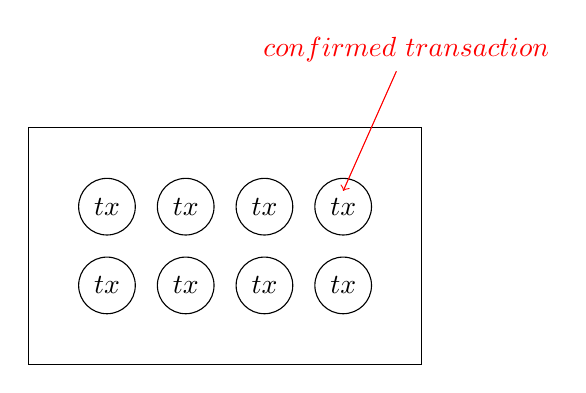
\begin{tikzpicture}
      \draw (0,0) rectangle (5,3);
      \foreach \x in {1,2,...,4}
        \foreach \y in {1,...,2}
          \node[circle,draw, minimum size=0.4cm] at (\x,\y) {$tx$};

      \node[red] (confirm) at (4.8, 4) {$confirmed \text{ }transaction$};
      \draw [->, red] (confirm) -- (4,2.2);
    \end{tikzpicture}
    \caption{A block}
    \label{fig:block:a}
  \end{subfigure}
  \begin{subfigure}[t]{0.50\textwidth}
    \centering
    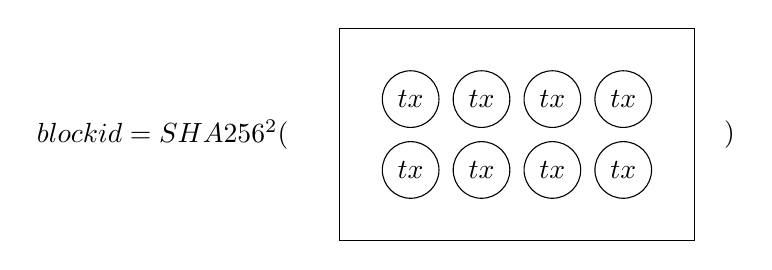
\begin{tikzpicture}[scale=0.9]
      \draw (0,0) rectangle (5,3);
      \foreach \x in {1,2,...,4}
        \foreach \y in {1,...,2}
          \node[circle,draw, minimum size=0.4cm] at (\x,\y) {$tx$};
      \node (txid) at (-2.5,1.5) {$blockid = SHA256^{2}($};
      \node (txid) at (5.5,1.5) {$)$};
    \end{tikzpicture}
    \caption{Bitcoin Block ID}
    \label{fig:block:b}
  \end{subfigure}
  \caption{Blocks}
  \label{fig:blocks}
\end{figure}

\begin{figure}[ht!]
  \centering
  \begin{tikzpicture}
    \foreach \x in {0,1,...,4}
        \pgfmathparse{(\x*3)}
        \edef\position{\pgfmathresult}
        \node[bl_block] (\x) at (\position,0) {$block$};

    \foreach \x in {1,2,...,4}
        \pgfmathparse{(\x-1)}
        \edef\previous{\pgfmathresult}
        \draw [->] (\x) -- (\previous);

  \end{tikzpicture}
  \caption{The blockchain}
  \label{fig:blockchain}
\end{figure}

\begin{figure}[ht!]
  \begin{tikzpicture}
    \foreach \x in {0,1,...,4}{
        \pgfmathparse{(\x*3)}
        \edef\position{\pgfmathresult}
        \node[bl_block] (\x) at (\position,0) {$block$};
        \pgfmathparse{int(\x*10 + 10)}
        \edef\time{\pgfmathresult}
        \node[] at (\position,-2) {$17:\time$};
    }


    \foreach \x in {1,2,...,4}
        \pgfmathparse{(\x-1)}
        \edef\previous{\pgfmathresult}
        \draw [->] (\x) -- (\previous);

    \node[ellipse, draw, red, inner xsep=6ex,inner ysep=3ex] (old_ell) at (0) {};
    \node[ellipse, draw, red, inner xsep=6ex,inner ysep=3ex] (recent_ell) at (4) {};
    \node[red,below=0cm of old_ell] (old) {$oldest\text{ }block\text{ }$};
    \node[red,below=0cm of recent_ell] (recent) {$recent\text{ }block\text{ }$};
  \end{tikzpicture}
  \caption{The blockchain timeline}
  \label{fig:blockchain_timeline}
\end{figure}

\section{Consensus mechanisms}\label{blockchain:consensus_mechanisms}

With the use of the blockchain data structure we manage to have chronological order of the transactions. What remains is a global agreement on order of the blocks among the participants of the network. Someone can easily change the order of two blocks within the chain by changing the respective hashes or producing new ones wherever required~\cite{zindros_thesis}. This would allow an adversary to fake the order of transactions in time, which is an undesired outcome.

The global agreement on a common truth, the global blockchain, is called consensus---a single universal “truth”--- and this is where Bitcoin's novelty is. The consensus mechanism is the core mechanism of the blockchain. Through consensus, the shared state of the ledger comes to an agreement upon a global state, allowing all the nodes of the network to reach the same ledger state. That is, the users of the network agree on a common order of the blocks in the blockchain and therefore on the order of the transactions. Achieving consensus in a distributed system is challenging. A consensus mechanism has to be resilient to node failures, network delays and the existence of malicious nodes.

At high level, every public consensus mechanism works as follows: A ``game'', involving randomness, is taken place where each node of the network participates. The winner of the game is eligible to propose the new block that will be adopted in the blockchain. This is a simple, but marvellous idea. The probabilistic nature of the process is paramount to its security.

There are three basic consensus mechanism categories:

\begin{enumerate}
  \item Proof-of-Work (PoW).
  \item Proof-of-Stake (PoS).
  \item Practical Byzantine Fault Tolerance (PBFT)
\end{enumerate}


\subsection{Proof of Work (PoW)}\label{blockchain:consensus:pow}

A Proof-of-Work (PoW) consensus mechanism, is a consensus mechanism where each node of the network tries to solve a computational puzzle that is computational hard, but feasible to find, and easy to verify correctness. Assuming that hash functions are hard to invert, proof of work usually is established by seeking a range-collision of the hash function on the block~\cite{zindros_thesis}.

\begin{figure}[!ht]
  \centering
  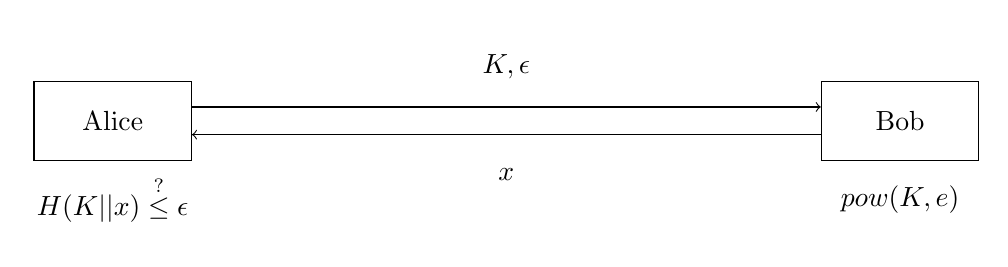
\begin{tikzpicture}[node distance=10cm, minimum height=1cm, minimum width=2cm]
    \node[draw] (a) {Alice};
    \node[draw, right of =a] (b) {Bob};
    \node[below of=a, node distance=1cm] (c) {$H(K || x) \stackrel{?}{\leq} \epsilon$};
    \node[below of=b, node distance=1cm] (d) {$pow(K, e)$};
    \draw[->] ([yshift=0.5em]a.east) -- ([yshift=0.5em]b.west) node[midway, above] {$K, \epsilon$};
    \draw[<-] ([yshift=-0.5em]a.east) -- ([yshift=-0.5em]b.west) node[midway, below] {$x$};
  \end{tikzpicture}
  \caption{The Proof-of-Work protocol}
  \label{fig:consensus:pow}
\end{figure}

Bitcoin~\cite{Zohar:2015:BUH:2817191.2701411} is the first blockchain system that utilizes a PoW for blockchain block generation. It work as follows: A target $\epsilon$ is given and is asked that the hash of the block is smaller than the target. The node can only modify a nonce, which is concatenated with the rest of the block data. By changing the nonce the node can change the block hash. As cryptographic hash functions is assumed to be one-way, the only way to find a hash value smaller than the target is with a series of brute-force trials of different nonce values. Bitcoin's proof-of-work can be summarized as:

\begin{equation*}
  H(txs || nonce || parent\_blockid) \leq \epsilon
\end{equation*}

The network evaluates collectively the target value using a predefined algorithm. That way, the network can control the difficulty of proof-of-work and the expected frequency of block generation is controlled. In Bitcoin the expected rate is one block per 10 minutes.

All the nodes of the network simultaneously try to produce a new block, meaning trying to find a correct nonce satisfying the proof-of-work requirements. Each node monitors the network for blocks and transactions while preparing its block. In its block the node includes all the valid transactions that are not in a previous block and a reference to a parent block. Every node of the network can produce a valid block but each block has to meet the target proof-of-work requirements.

When a hash value less than the target is found by a node, the node gets to add the proposed block to the blockchain and broadcast the new block to to all its neighbours which, in turn, transmit it to the whole network. If a block is found by another node, all the nodes stop the proof of work procedure and start over upon the new block. For a block to be accepted as valid it must contain valid transactions, a valid proof-of-work and a reference to a known valid parent block.

The existence of a transaction in a block makes the transaction valid. The deeper the block is in the blockchain the more difficult is for an adversary to alter the block in which the transaction is confirmed. The reason is, that the time an adversary needs to alter a block grows exponentially in the number of blocks that have followed~\cite{10.1007/978-3-662-46803-6_10}, as she will need to reproduced those blocks and the blockchain is constantly extended. Waiting 6 confirmation blocks to appear after the block in which the transaction is confirmed is enough for a transaction to considered secure.

A PoW system is based on randomness. Each node has a small change to win the block which is approximated proportionally to the computational power of each node. The consensus mechanism depends on having a majority of the miners acting honestly out of self-interest~\cite{antonopoulos2014mastering}.

PoW consensus mechanism works very well in public blockchain systems where trust of the nodes is low eliminating the double-spend problem and guarding against Sybil attacks~\cite{Vu:2009:PCP:1671222}. However, the transaction confirmation time is longer compared to conventional financial services (such as VISA)~\cite{Sompolinsky2015,Zohar:2015:BUH:2817191.2701411,DBLP:journals/corr/abs-1708-05665} resulting in slower transaction confirmation rates. Lastly, the energy waste attributed to the mining process can be very high ---the energy requirements of the Bitcoin protocol are estimated to be comparable to those of a small country~\cite{6912770}.

\begin{lstlisting}[language=C, caption={A simple Proof-of-Work Algorithm}, mathescape=true]
  x = rand();

  do {
    ++x;
  } while (H(K||x) >= $\epsilon$);

  return x;
\end{lstlisting}

\subsection{Proof of Stake (PoS)}\label{blockchain:consensus:pos}

Proof-of-Stake algorithms are designed to overcome the disadvantages of PoW in terms of the high electricity consumption involved in mining~\cite{bl_consensus}
and provide equal security guarantees~\cite{Kiayias2017}. Unlike PoW where the nodes of the network solve computational puzzles in order to create a new block, in PoS the choice
of the block creator among the miners is random, yet relative to the stake the node possesses according to the current blockchain ledger. Maintaining
the blockchain relies on the stakeholders themselves and assigns work to them based on the amount of stake that each possesses as reported in the ledger~\cite{Kiayias2017}. The higher the stake participant, the higher the possibility to be chosen.

Proof-of-Stake algorithms suffer from the so-called “nothing at stake” problem. The “nothing at stake” problem refers to attacks against PoS blockchain systems where shareholders do not have
incentives to follow the protocol and vote simultaneously on multiple blockchains exploiting the fact that little computational effort
is needed to build a PoS blockchain~\cite{Kiayias2017}. Ouroboros is the first provable secure PoS algorithm~\cite{Kiayias2017} and is the main consensus algorithm of the Cardano blockchain~\cite{cardano_site}.

\subsection{Practical Byzantine Fault Tolerance (PBFT)}\label{blockchain:consensus:PBFT}

The Practical Byzantine Fault Tolerance algorithm~\cite{Castro:1999:PBF:296806.296824} is the first practical consensus algorithm with Byzantine Fault Tolerance~\cite{byzantine_fault_tolerance}.
It is based on the concept of state machine replication and replication state voting, and is able to process tens of thousands of requests per second with minimal latency.
The algorithm has only a 3\% overhead over a typical filesystem~\cite{Castro:1999:PBF:296806.296824}.

PBFT and state-machine replication protocols’ downside is related to scalability, in terms of the number of nodes (replicas)~\cite{Vukolić2016} that can be supported.
PBFT has only been scaled and studied up to 20 replicas~\cite{bl_consensus,Vukolić2016}. To overcome this limitation, without compromising security, various PBFT variants,
such as Ripple and Stellar, partition the network into smaller groups called federates and each one runs a local consensus protocol among its members and
global consensus is achieved when certain conditions are being met~\cite{DBLP:journals/corr/abs-1708-05665}.

\begin{table}[!ht]
  \centering
  \begin{tabular}{|l|l|l|l|}
    \hline
    & PoW &	PoS &	PBFT \\ \hline
    Blockchain Type &	Permissionless &	Both &	Permissioned \\ \hline
    Scalability of nodes &	High &	High &	Low \\ \hline
    Scalability of clients &	High &	High &	High \\ \hline
    Transaction rate &	Low &	High &	High \\ \hline
    Latency &	High &	Low &	Minimal \\ \hline
    Power consumption &	High &	Low &	Low \\ \hline
    Token needed &	Yes &	Yes &	No \\ \hline
    Cost of participation &	Yes &	Yes &	No \\ \hline
    Adversary tolerance &	$\leq$ 25\%	& Depends &	$\leq$ 33\% \\ \hline
  \end{tabular}
  \caption{Blockchain consensus mechanisms. Adapted and modified from~\cite{bl_consensus,Vukolić2016}}
  \label{table:blockchain_consensus}
\end{table}

\section{Mining \& incentives}\label{blockchain:mining}

The process of creating a block in a PoW consensus system is known as mining and the participants as miners. The first block was mined by Satoshi Nakamoto~\cite{nakamoto2012bitcoin} and is called the genesis block. Every valid chain starts from the genesis block.

For miners to participate in the network and contribute their computation resources incentives are provided. Normally, in a permissionless blockchains such as Bitcoin or Ethereum a monetary incentive in the form of cryptocurrency incentivize the miners and in a permissioned blockchain finance incentives or access to blockchain data could encourage miners to participate~\cite{deloitte}.

In Bitcoin, the miner is rewarded with a number of bitcoins that are created for the specific block. This happens through a specific type of transaction called \textbf{coinbase}. This type of transaction has an unconnected income edge without a sender and an outcoming edge with recipient the miner that found the particular block. This is how new bitcoin is generated. The amount of coin mined in each block is preagreed on by the network and every four years is reduced by half. Currently, the reward is 12,5 BTC.

\begin{figure}[!ht]
  \centering
  \begin{tikzpicture}
    \node[tx] (A) at (0,0) {$tx$};
    \draw [->] (-3,0) -- (A) node[midway, below]{} node[midway, above]{12.5 BTC};
    \draw [->] (A) -- (3, 0) node[midway, below]{miner} node[midway, above]{12.5 BTC};
  \end{tikzpicture}
  \caption{Coinbase transaction}
  \label{fig:mining:coinbase}
\end{figure}

Another way a miner is rewarded is by collecting transactions fees;  the financial remain of a confirmed transaction. This can happen when a user makes a transaction where the total value of all incoming edges are bigger than the total value of all outcoming edges. In particular the total fees of a block are defined as:

\begin{equation*}
  fees = \sum_{tx \in block} [ \sum_{i \in in(tx) }w(i) -  \sum_{o \in out(tx) }w(o)]
\end{equation*}

\section{Blockchain fork}\label{blockchain:fork}

Due to network latency and the distributed nature of the system, it is possible that two miners will find a block around the same time and some nodes will accept the first block and some others the second one. Both blocks are valid, containing a valid proof of work, valid transactions and both extent the same parent block. In such cases there is a temporary fork in the blockchain, where some nodes are adding blocks to one branch while other nodes are adding blocks to another branch. As a result, two competitive versions of the blockchain will emerge~\cite{antonopoulos2014mastering}. This situation, arise the same problem we have with the transactions: the order of the blocks cannot be defined.

To resolve this, each node always selects the longest brach. At some point, one of the two branches will be extended by a new block. The nodes that were working on the first branch will see that the new branch is the longest and start working immediately on that. Eventually the system will come to an agreement, the longest branch will be accepted and the others will be discarded. The process of chain selection can be likened to voting where mining nodes ``vote'' with their mining power by choosing which chain to extend by mining the next block; the new block itself represents the voting result~\cite{antonopoulos2014mastering}.

\begin{figure}[!ht]
  \centering
  \begin{tikzpicture}
    \foreach \x in {0,1,...,5}
        \pgfmathparse{(\x*2)}
        \edef\position{\pgfmathresult}
        \node[bl_block, minimum width=1cm, fill=blue!30] (\x) at (\position,0) {$block$};

    \foreach \x in {1,2,...,5}
        \pgfmathparse{(\x-1)}
        \edef\previous{\pgfmathresult}
        \draw [->] (\x) -- (\previous);

    \foreach \x in {3,4}
        \pgfmathparse{(\x*2)}
        \edef\position{\pgfmathresult}
        \node[bl_block, minimum width=1cm, fill=orange!30] (\x_fork) at (\position,2) {$block$};

    \draw [->] (4_fork) -- (3_fork);
    \draw [<-] (2.north) -- (3_fork.west);

  \end{tikzpicture}
  \caption{A blockchain fork}
  \label{fig:bl:fork}
\end{figure}

If a malicious adversary wants to do create double spent transactions or execute a denial-of-service, she has to produce a malicious blockchain longer than the honest. To achieve that, an adversary would need to control the majority of the CPU power of the network and specifically the 51\% of the total network’s hashing power. This is called the 51\% attack. It is important to node that this kind of consensus attack affects at best the most recent blocks. Beyond a certain depth blockchain is absolute immutable. In addition, this type of attacks cannot steal or spend coins as the adversary has to forge a signature to produce a valid transaction impersonating another user.

 Bitcoin's security has been formalized and rigorously explored~\cite{10.1007/978-3-662-46803-6_10} over the last years.

\begin{figure}[ht!]
  \centering
  \begin{tikzpicture}
    \foreach \x in {0,1,...,5}
        \pgfmathparse{(\x*2)}
        \edef\position{\pgfmathresult}
        \node[bl_block, minimum width=1cm, fill=blue!30] (\x) at (\position,0) {};

    \foreach \x in {1,2,...,5}
        \pgfmathparse{(\x-1)}
        \edef\previous{\pgfmathresult}
        \draw [->] (\x) -- (\previous);

    \foreach \x in {3,...,6}
        \pgfmathparse{(\x*2)}
        \edef\position{\pgfmathresult}
        \node[bl_block, minimum width=1cm, fill=red!30] (\x_mal) at (\position,2) {};

    \draw [->] (4_mal) -- (3_mal);
    \draw [->] (5_mal) -- (4_mal);
    \draw [->] (6_mal) -- (5_mal);

    \draw [<-] (2.north) -- (3_mal.west);

    \node[circle, draw, minimum size=0.1cm, fill=red] at (4_mal.center) {};
    \node[circle, draw, minimum size=0.1cm, fill=green] at (3.center) {};

    \draw[decorate,decoration={brace,amplitude=10pt, mirror}, xshift=-1.2em, yshift=-1.5em](0, 0) -- (5, 0) node [black,midway,yshift=-1cm, above] {\footnotesize{Honest common prefix}};

    \draw[decorate,decoration={brace,amplitude=10pt, mirror}, xshift=-1.2em, yshift=-1.5em](6, 0) -- (11, 0) node [black,midway,yshift=-1cm, above] {\footnotesize{Honest blockchain}};

    \draw[decorate,decoration={brace,amplitude=10pt}, xshift=-1.2em, yshift=1.5em](6, 2) -- (13, 2) node [black,midway, above, yshift=1em] {\footnotesize{Malicious blockchain}};

  \end{tikzpicture}
  \caption{Double spent attack}
  \label{fig:blockchain:dl_spent}
\end{figure}

\section{Blockchain Types}\label{blockchain:blockchain_types}

There are various types of blockchains varying in restrictions on data access and participation in the consensus process. Each one has its own advantages and disadvantages.

\begin{itemize}
  \item Public Blockchain: A public blockchain is a blockchain, in which there are no restrictions on reading blockchain data -encrypted or not- and validating transactions~\cite{prbc_vs_pubbc}.
  The most common implementation of a public blockchain is Bitcoin~\cite{nakamoto2012bitcoin} and Ethereum~\cite{ethash}.
  \item Federated or Consortium blockchain: In a federated blockchain transaction validation is limited to a predefined list of entities with their identities known to the network. Data access can either be public or restricted~\cite{prbc_vs_pubbc}.
  \item Private blockchain: A private blockchain is a blockchain where consensus mechanism is centralized to one single entity regardless of data access~\cite{prbc_vs_pubbc}.
\end{itemize}

\section{Consensus defined types of Blockchain}\label{blockchain:consensus_blockchain_types}

\begin{itemize}
  \item Permissionless blockchain: A permissionless blockchain is a blockchain, in which there are no restrictions on identities of transaction processors (i.e., users that are eligible to create blocks of transactions)~\cite{prbc_vs_pubbc}.
  \item Permissioned blockchain: A permissioned blockchain is a blockchain, in which transaction processing is performed by a predefined list of subjects with known identities~\cite{prbc_vs_pubbc}.
\end{itemize}

\begin{table}[!ht]
  \centering
  \begin{tabular}{|l|l|l|l|}
    \hline
     & Public & \makecell[cl]{Permissioned \\ (Multiple Entities)} & \makecell[cl]{Private \\ (Single Entity)} \\ \hline
     Participants & \makecell[cl]{Permissionless \\ Anonymous} & \makecell[cl]{Permissioned \\ Identified \\ Trusted} & \makecell[cl]{Permissioned \\ Identified \\ Trusted} \\ \hline
     Data Access & Public & Public or Restricted & Restricted \\ \hline
     Consensus & PoW, PoS & FBTA, PoS & FBTA \\ \hline
  \end{tabular}
  \caption{Blockchain Types. Source~\cite{hub-bl-types}}
  \label{table:blockchain_types}
\end{table}

\section{Blockchain Implementations}\label{blockchain_implementations}

\subsection{Bitcoin}\label{blockchain:impl:bitcoin}

Bitcoin is the first decentralized digital currency. The main currency is called Bitcoin and is used to store and transmit value among participants in the Bitcoin network. The Bitcoin network is a fully distributed peer-to-peer network where anyone can freely join running an open source implementation of the bitcoin protocol and there is no need for trust to the network; in the network any node may be malicious. As a result, Bitcoin is a public permissionless blockchain. Bitcoin's use a Proof-of-Work consensus mechanism for keeping consistent the public ledger, preventing double spend and confirm transactions. Bitcoin is the oldest digital currency decentralized network running from 3 January 2009~\cite{btc_first_block}. As a result, Bitcoin is the most well studied Blockchain network~\cite{10.1007/978-3-662-46803-6_10} with various published papers on different topics such as privacy~\cite{10.1007/978-3-319-70278-0_8, 10.1007/978-3-642-39884-1_2, Bonneau14e.w.:mixcoin, 10.1007/978-3-662-44774-1_9}, economics~\cite{Babaioff:2012:BRB:2229012.2229022, 10.1007/978-3-319-70278-0_17, Bentov2017DecentralizedPM, Carlsten:2016:IBW:2976749.2978408}, attacks~\cite{DBLP:journals_corr_Bahack13, DBLP:journals_corr_EyalS13}, network~\cite{10.1007/978-3-662-44774-1_7, 190890} and scalability~\cite{kiayias2017non, 10.1007/978-3-662-53357-4_5, 10.1007/978-3-662-53357-4_8}. Due to the years Bitcoin's blockchain has grow significantly is size making difficult to some devices to store the entire blockchain and run as a full node leading to network centralization. Specifically, as of April 2018 the Bitcoin's blockchain size is over 160GB~\cite{btc_bl_size}.

Bitcoin suffers from scalability due to the limit on the amount of transactions the bitcoin network can process. The transaction processing capacity maximum is estimated between 3.3 and 7 transactions per second~\cite{10.1007/978-3-662-53357-4_8}. The limit is related to the block size limit---the total number of transactions a block can contain--- that was introduces as an anti-spam measure. There are various proposed and activated solutions to address this issue. One activated solution is Segregated Witness (SegWit, BIP 141)~\cite{segwit} which performed as a soft fork and increased the block size by a factor of approximately of two.

As of April 2018, Bitcoin is the most widely used crypto currency~\cite{10.1007/978-3-642-39884-1_2} with over of 100,000 merchants that accept Bitcoin~\cite{btc_merchants} and with the biggest total market cap~\cite{btc_cap}.

\subsection{Ethereum}\label{blockchain:impl:ethereum}

Ethereum is an open-source, public, blockchain-based distributed computing platform featuring smart contract functionality.
It provides a decentralized Turing-complete virtual machine, the Ethereum Virtual Machine (EVM), which can execute scripts using an
international network of public nodes~\cite{ethereum_yellowpaper}. Ethereum provides a cryptocurrency called ether which can be transferred between accounts, and gas, an internal pricing mechanism used to execute contracts and allocate resources on the network. Through EVM, Ethereum provides Solidity a Turing-complete language for writing smart contracts that enables anyone to build distributed applications making the process much easier and efficient than ever before. Ethereum use a Proof-of-Work consensus mechanism called Ethash and has been designed to be ASIC-resistant~\cite{ethash}.
Soon Ethereum will be moved to a Proof-of-Stake consensus mechanism called Casper. Ethereum can be implemented as well as a permissioned blockchain~\cite{consortium_chain_development,quorum}.

\subsection{Cardano}\label{blockchain:impl:cardano}

Cardano is a security focused blockchain that utilize the latest research and engineering insights to build a platform suitable for
the highest value applications~\cite{cardano_site}. It supports distributed applications creation and smart contracts verifiable by a method called formal
verification allowing logical proof of correctness of code providing high security. Cardano addresses the need for regulatory oversight while
maintaining consumer privacy and security. Cardano is the first blockchain project to be peer reviewed by academic researchers~\cite{cardano_site} and its consensus
mechanism, Ouroboros, is the first Proof of Stake algorithm to be provably secure~\cite{Kiayias2017}.
Cardano consists of two main layers, one for accounting and one for computation. The accounting layer is called Cardano Settlement Layer (CSL)
and the computation layer Cardano Computation Layer (CCP) where distributed application can be built and run upon. The CCP layer has not been
implemented yet and there is a plan to be released as a beta by the first quarter of 2018~\cite{cardano_parsons}.

\section{Smart Contracts}
\label{smart_contracts}

A smart contract is a computer protocol intended to facilitate, verify, or enforce the negotiation or performance of a contract~\cite{FM548,szabo1996smart}.
The idea of smart contracts proposed in the early 1990s~\cite{FM548}, by Nick Szabo, and have been used primarily in association with cryptocurrencies enabling
parties to formally specify a cryptographically enforceable agreements~\cite{7163021}. A smart contract consists of a set of promises including protocols within which the parties perform on these promises. It can define rules and penalties around an agreement and automatically enforce those obligations. The contractual rules may be partially or fully self-executed, self-enforcing or both. On blockchain technologies a smart contract is any computer program that is executed on the blockchain---a general purpose computation.

Bitcoin is the first blockchain that provides a scripting language for expressing simple smart contracts such as ownership of an amount of coins by one or multiple entities. Bitcoin's language is a stack-based scripting language inspired by Forth~\cite{forth_lang} and offers a set of simple serial commands supporting cryptographic primitives such as hash functions and signature verification. The main disadvantage of Bitcoin's language is that is not Turing-complete limiting the type of smart contracts one can create. Furthermore, adding new commands to extent functionality requires either a soft-fork which has to be decided by the majority of bitcoin network or to fork Bitcoin's code and implement a new blockchain supporting the new features in which the Bitcoin's network power is lost. Numerous previous smart contract application atop Bitcoin (e.g., lottery\cite{Andrychowicz:2014:SMC:2650286.2650764,10.1007/978-3-662-44381-1_24},
verifiable computation~\cite{Kumaresan:2014:UBI:2660267.2660380}) have demonstrated the difficulty of Bitcoin's scripting language~\cite{cryptoeprint:2015:675}.

The need of user defined open source blockchain applications emerged. As a result, Ethereum was born which is the first Turing-complete decentralized smart contract framework. In Ethereum, one can create smart contracts in a high level language such as Solidity~\cite{solidity} which in turn is compiled to bytecode that is executable on the Ethereum.

With Ethereum launch, the notion of DApps (decentralized applications) arisen
and a lot of developers and companies are building numerous applications atop Ethereum such as prediction markets~\cite{augur,gnosis}, social media platforms~\cite{akasha,backfeed},
online gambling~\cite{etheroll,coinpoker} and video games~\cite{cryptokitties}. As of January 2018, there are more than 250 live DApps, with hundreds more under development.

\clearpage

\begin{lstlisting}[language=Solidity, caption={An Ethereum Smart Contract}]
pragma solidity ^0.4.16;

contract Namespace{

  struct NameEntry {
      address owner;
  }

  uint32 constant REGISTRATION_COST = 100;
  uint32 constant UPDATE_COST = 10;
  mapping(bytes32 => NameEntry) data;

  function nameNew(bytes32 hash){
      if (msg.value >= REGISTRATION_COST){
          data[hash].owner = msg.sender;
      }
  }

  function nameUpdate(bytes32 name, bytes32 newValue, address newOwner){
      bytes32 hash = sha3(name);
      if (data[hash].owner == msg.sender && msg.value >= UPDATE_COST) {
          data[hash].value = newValue;
          if(newOwner != 0) {
              data[hash].owner = newOwner;
          }
      }
  }

  function nameLookup (bytes32 name) {
      return data[sha3(name)]
  }
}
\end{lstlisting}

\clearpage

%!TEX root = ../thesis.tex
\chapter{Problem Statement}
\label{problem}

The amount of data is rapidly increasing and it is estimated that 20\% of the world's data have been collected the past
few years~\cite{10.1109/SPW.2015.27,big_data_better_worse}. People constantly producing and publishing data about themselves
leaving a constant moving digital fingerprint over the Internet--their personal data. The type, quantity and value of personal data
being collected are vast~\cite{emergence_new_assets_wef}: banks accounts, medical records, employment data, web searches, sites visited,
likes, dislikes, product purchase histories, quotes, tweets, texts, emails, phone calls, photos, videos, personal moments, emotions
as well as coordinations of real-world locations.


\section{Data trading}\label{problem:data_trading}

~\cite{emergence_new_assets_wef}

\section{Regulations}\label{problem:regulations}

The recent approval of the new General Data Protection Regulation (GDPR)~\cite{gdpr} in 2016 by the European Commission (EC)
imposes new obligations on data controllers and processors in contrast to the previously adopted Data Protection Directive (DPR)~\cite{eu-46ec-1995}.
New legislation aims in the extension of responsibility and accountability requirements of organizations also demanding explicit
consent of the data subjects (person) securing their right to withdraw, and to be forgotten~\cite{DBLP:journals/corr/NeisseSF17}.

The key changes of the new data protection law introduced by the GDPR in contrast to the DPR is are~\cite{DBLP:journals/corr/NeisseSF17}:
\begin{itemize}
    \item Organisations based outside EU that process personal data of EU residents are applicable to the new legislation
    \item All EU member states are obliged to a single set of rules
    \item The responsibility and accountability requirements of organisations are extending
    \item EU residents are empowered with explicit consent over their data with the right to be forgotten
\end{itemize}



\section{Motivations for applications}\label{problem:motivations}

banking, healthcare, national security, citizenship documentation or online retailing

%!TEX root = ../thesis.tex
\chapter{Solution}
\label{solution}

In our solution a public blockchain is used as the controller of the application. It is responsible for keeping an
audit, immutable, tamper-proof and transparent log of all actions of the participants.

Blockchain does not provides an extra security layer concerning datasets. The datasets are stored off-chain, data controllers are responsible for the security of their system and the participants can still collaborate outside the Blockchain network. Nevertheless, the use of the Blockchain can guarantee accountability, auditability and provenance tracking of the data increasing the trust for the system.

\section{Participants}
\label{solution:entities}

There are three main roles consisting the application: the data controller, the data processor
and the data requester. The first two are also defined in the context of GDPR (§~\ref{problem:regulations}).
GDPR defines another role, that of data subject; the owner of the data.
In our scheme we assume that the data controller already has consent to access or forward the data or she is at the same time the data subject and the data controller.

\subsection{Data Controller}
\label{solution:entities:data_controller}

The data controller is in charge of a data set. She run on behalf of a data subject (person)
that authorizes the data controller to access her personal data, with the possibility of forwarding
them to a data processor that will be responsible for processing the data on behalf of controller~\cite{DBLP:journals/corr/NeisseSF17}.

\subsection{Data Processor}
\label{solution:entities:data_processor}

The data processor is responsible for processing data on behalf of the data controller. She listens for data processing requests and returns, along with the output of the process, a Zero Knowledge Proof of correct computation over the requested data set.

\subsection{Data Requester}
\label{solution:entities:data_req}

The requester can be any entity that requests a computation over a data set. It can be a research center, a university, a machine learning algorithm or any individual. The requester expects, along with the output, a proof of correct computation over the requested data set that verifies at the end of the processing.

\section{Trust model}
\label{solution:trust_model}

Before we explain in detail our architecture, we would like to introduce our thread model and what exactly our goals are. It is important to understand the possible roles of adversaries, their strengths and their resources.

In our model we assume that the involved entities that interact with a data set---the data controller and the data processor---are identified and verified through a public key infrastructure (PKI)~\cite{adams_understanding_2003}. Furthermore, each entity is a trusted entity with certain trust properties. In particular, the data controller is trusted for integrity and confidentiality and the data processor only for confidentiality.

Adversaries can be categories in 4 categories:

\begin{itemize}
  \item Malicious data controller
  \item Malicious data processor
  \item Malicious data requestor
  \item Malicious public user
\end{itemize}

\section{Algorithms}
\label{solution:algorithms}

The system should support only a set of open-source algorithms that have been analyzed and constructed to be privacy-preserving with the use of techniques such as k-anonymity~\cite{Samarati98protectingprivacy} and l-diversity~\cite{Aggarwal2008}. This algorithms should return only de-identified aggregated results.

The supported algorithms are:

\begin{enumerate}
  \item Sum
  \item Average
  \item Count
  \item Maximum
  \item Median
  \item Minimum
\end{enumerate}

The above algorithms are not considered to be privacy-preserving as it is outside the scope of the initial prototype and should be implemented on future work(§~\ref{future_work:ppq}).

\section{Flow}
\label{solution:flow}

\subsection{Dataset Registration}
\label{solution:flow:reg_data}

Naturally, for datasets to be available for processing a data registration process is needed. Anyone who register a dataset automatically becomes a data controller who is responsible for the availability and quality of the it. The dataset should be publicly available on any location of choice provided that the controller expose an API for data retrieval. The location can be in a distributed file system~\cite{ipfs}, a decentralized cloud storage~\cite{storj} or a central server. As long as the involved participants communicate over the same protocol the choice is irrelevant; the system can be agnostic concerning data storage.

The confidentiality of the dataset must rely solely on cryptographic primitives with strong guarantees. Therefore, every dataset is encrypted using the symmetric encryption algorithm \verb|AES| with \verb|256-bit| key length and \verb|CTR| as mode of operation. In addition, the hash of contents of the unencrypted dataset is computed using the cryptographic hash function \verb|SHA256|.

A dataset is actually registered and available when a \textbf{register} transaction is sent to blockchain, signed by the data controller. The transaction needs to include the name of the dataset, a category, the location (URI) and the checksum (hash) of the file. From the name of the dataset a unique persistent identifier is created, to which all participants refer to. Two datasets with the same name cannot be saved; the transaction is rejected in the case of name duplication.

The data registration procedure is summarized in Algorithm~\ref{alg:data_registration}.

\begin{algorithm}[!htb]
  \caption{Dataset registration}\label{alg:data_registration}
  \begin{algorithmic}[1]
  \Function{\sf save}{file}
      \Let{h}{H(file)}
      \Let{k}{\calg}
      \Let{c}{Enc_{k}(file)}
      \Let{uri}{store(c)}
      \State \Return{$(h, k, uri)$}
  \EndFunction
  \Function{\sf broadcast}{name, uri, category, hash}

        \Let{h_{meta}}{H(name || uri || category || hash)}
        \Let{tx}{(name, uri, category, hash, h_{meta})}
        \State $tx.send()$
        \State \Return{$tx$}
  \EndFunction
  \Procedure{\sf register}{name, file, category}
    \Let{(h, k, uri)}{save(file)}
    \Let{tx}{broadcast(name, uri, category, h)}
    \State \Return{$(tx, k)$}
  \EndProcedure
  \end{algorithmic}
\end{algorithm}

\begin{figure}[ht!]
  \begin{tikzpicture}
    \node[blockchain] (blockchain) at (0,0){Blockchain};

    \begin{scope}[node distance=4cm]
      \node[node, anchor=west] (owner) at (0,-5) {Data Controller};
      \node[database] (db) [below right=of owner] {Datastore};
      \draw[<->] (owner) -- (db) node[midway,left] {$Enc_k(data)$};
      \draw[<-] ([xshift=-1em]owner.north) -- ([xshift=-1em]2,-0.5);
      \draw[->] ([xshift=1em]owner.north) -- ([xshift=1em]2,-0.5) node[midway,right] {$Tx(\{name, location, category, digest, address, hashMeta\}, "register\_data")$};
    \end{scope}

  \end{tikzpicture}
  \caption{Data registration}
  \label{fig:arc:reg}
\end{figure}

\subsection{Entity Registration}
\label{solution:flow:entity_reg}

\begin{enumerate}
  \item Data controller generates an asymmetric encryption key pair
  \item A trusted entity registers data controller's availability by initiating a transaction that saves processors name and public key on the blockchain
\end{enumerate}

\begin{algorithm}[!htb]
  \caption{Entity registration}\label{alg:entity_registration}
  \begin{algorithmic}[1]
  \Procedure{\sf register\_entity}{name, $p_k$, address}
    \Let{tx}{(name, p_k, address)}
    \State $tx.send()$
    \State \Return{$tx$}
  \EndProcedure
  \end{algorithmic}
\end{algorithm}

\begin{figure}[ht!]
  \begin{tikzpicture}
    \node[blockchain] (blockchain) at (0,0){Blockchain};

    \begin{scope}
      \node[node, anchor=west] (controller) at (0,5) {PKI};
      \draw[<-] ([xshift=-1em]controller.south) -- ([xshift=-1em]2,0.5);
      \draw[->] ([xshift=1em]controller.south) -- ([xshift=1em]2,0.5) node[midway,right] {$Tx(\{name, pubKey, address\}, "register\_entity")$};
    \end{scope}

  \end{tikzpicture}
  \caption{Entity Registration}
  \label{fig:arch:entity_reg}
\end{figure}



\subsection{Request for processing}
\label{solution:flow:pr_req}

\begin{enumerate}
  \item The requestor selects a data set on which the processing should be made and  notify the network participants of the request by initiating a transaction on the blockchain passing along her public key
\end{enumerate}

\begin{algorithm}[!htb]
  \caption{Request for processing}\label{alg:data_request}
  \begin{algorithmic}[1]
  \Function{\sf notify}{$e$}
    \State $p \rselect \{ p_1, p_2, \dots p_n \}$ \Comment{Select randomly processor}
    \Let{(requestID)}{e}
    \Let{tx}{(p)}
    \Let{(pk_p)}{tx.send()} \Comment{Get processor public key}
    \Let{c}{Enc_{pk_p}(k)} \Comment{Encrypt symmetric key}
    \Let{tx}{(requestID, c)}
    \State $tx.send()$
    \State \Return{$tx$}
  \EndFunction
  \Procedure{\sf request}{datasetID, algorithmID, $p_{k}$}
    \Let{tx}{(datasetID, algorithmID, p_{k})}
    \State $tx.send()$
    \State \Return{$tx$}
  \EndProcedure
  \Procedure{\sf watch}{\null}
    \While{$e \in$ events['request']} \Comment{Listen data processing requests}
      \CommentLine{Check if the controller is the owner of the dataset}
      \If{isOwner($e$.datasetOwner)}
        \State notify($e$) \Comment{Notify processor}
      \EndIf
    \EndWhile
  \EndProcedure
  \end{algorithmic}
\end{algorithm}

\subsection{Handle request for processing}
\label{solution:flow:handle_request}

\begin{enumerate}
  \item The controller, responsible for the desired data set, selects a processor and encrypts the symmetric key with the public key of the selected processor
  \item The controller notifies the processor by initiating a transaction on the blockchain passing all needed information such as the encrypted symmetric key and the request ID.
\end{enumerate}

\begin{figure}[ht!]
  \begin{tikzpicture}

    \node[blockchain] (blockchain) at (0,0){Blockchain};

    \begin{scope}[node distance=4cm]
      \node[node, anchor=west] (owner) at (0,-5) {Data Controller};
      \draw[->] ([xshift=0em]owner.north) -- ([xshift=0em]2,-0.5);
    \end{scope}

    \node[txt] (list_req) [below=of owner, xshift=0em, yshift=1.5em] {$listen("request\_processing")$};

    \begin{scope}
      \node[node, anchor=west] (processor) at (0,5) {Data Processor};
      \draw[<-] ([xshift=0em]processor.south) -- ([xshift=0em]2,0.5) node[midway,right] {$Tx(\{requestID, Enc_{pk_P}(k)\}, "notify\_processor")$};
    \end{scope}

    \node[txt] (list_req_cr) [above=of processor, xshift=0em, yshift=-1.5em] {$listen("processing")$};

    \begin{scope}
      \node[node, anchor=east] (requester) at (\textwidth,-5) {Requester};
      \draw[->] ([xshift=0em]requester.north) -- ([xshift=0em]14.45,-0.5) node[midway,left] {\small $Tx(\{dataSetID, queryID, pubKey\}, "request\_processing")$};
    \end{scope}

  \end{tikzpicture}
  \caption{Request for processing}
  \label{fig:arch:req_pr}
\end{figure}

\subsection{Dataset processing}
\label{solution:flow:pr_data}

A data processor:

\begin{enumerate}
  \item Get the symmetric key
  \item Decrypt the data set
  \item Process the data
  \item Creates a Zero Knowledge Proof (§~\ref{zkp}) of the correctness of the computation for the specific dataset
  \item Encrypts the results with the public key of the requestor
  \item Submits the encrypted result of the computation on the Blockchain along with the proof.
\end{enumerate}

\begin{algorithm}[!htb]
  \caption{Dataset processing}\label{alg:data_processing}
  \begin{algorithmic}[1]
  \Function{\sf zkp}{$d$, algorithmID, $h$}
    \Let{valid}{false}
    \Let{h^{'}}{H(d)} \Comment{Get the digest of the dataset}
    \If{$h^{'} == h$} \Comment{Check if the digest match}
      \Let{valid}{true}
    \EndIf
    \Let{y}{\textsf{Compute($d$)}} \Comment{Process dataset}
    \State \Return{$(\pi, y, valid)$} \Comment{Return results}
  \EndFunction
  \Procedure{\sf process}{e}
    \Let{(requestID, algorithmID, c_{k}, pk_r)}{e}
    \Let{tx}{(requestID)}
    \Let{(datasetID, location, h)}{(tx)} \Comment{Get dataset info}
    \Let{k}{Dec_{sk_{p}}(c_{k})} \Comment{Decrypt symmetric key}
    \Let{c_{d}}{get(location)} \Comment{Get encrypted dataset}
    \Let{d}{Dec_{k}(c_{d})} \Comment{Decrypt dataset}
    \CommentLine{Process dataset and get proof of computation}
    \Let{(\pi, y, valid)}{zkp(d, algorithmID, h)}
    \Let{tx}{(H(\pi), Enc_{pk_r}(\pi, y, valid))} \Comment{Send results to requestor}
    \State $tx.send()$
  \EndProcedure
  \Procedure{\sf watch}{\null}
    \While{$e \in$ events['process']} \Comment{Listen data processing notifications}
      \State process($e$) \Comment{Process request}
    \EndWhile
  \EndProcedure
  \end{algorithmic}
\end{algorithm}

\begin{algorithm}[!htb]
  \caption{Proof verification}\label{alg:data_verify}
  \begin{algorithmic}[1]
  \Procedure{\sf verify}{e}
    \Let{(requestID)}{e}
    \Let{tx}{(requestID)}
    \Let{(proof)}{(tx)} \Comment{Get request info}
    \Let{(h, c)}{proof}
    \Let{(\pi, y, valid)}{Dec_{sk_{r}}(c)} \Comment{Decrypt results}
    \Let{result}{\_verify(\pi, y ,valid)} \Comment{Verify proof}
    \If{!valid || !result} \Comment{Reject if not valid}
      \State \textbf{reject}
    \EndIf
  \EndProcedure
  \Procedure{\sf watch}{\null}
    \While{$e \in$ events['process\_done']} \Comment{Listen data processing completion}
      \State verify($e$) \Comment{Process request}
    \EndWhile
  \EndProcedure
  \end{algorithmic}
\end{algorithm}

\begin{figure}[ht!]
  \begin{tikzpicture}

    \node[blockchain] (blockchain) at (0,0){Blockchain};

    \begin{scope}
      \node[node, anchor=west] (processor) at (0,5) {Data Processor};
      \draw[->] ([xshift=0em]processor.south) -- ([xshift=0em]2,0.5) node[midway,right] {$Tx(\{requestID, Enc_{pk_R}(\pi, y)\}, "notify\_requester")$};
    \end{scope}

    \node[node, process] (compute) [above of=processor, yshift=3cm] {$Compute$};

    \draw[->] ([xshift=-1em]compute.south) -- ([xshift=-1em]2,5.5) node[midway,left] {$(y, \pi)$};
    \draw[<-] ([xshift=1em]compute.south) -- ([xshift=1em]2,5.5)  node[midway,right] {$dataset$};

    \begin{scope}
      \node[node, anchor=east] (requester) at (\textwidth,-5) {Requester};
      \draw[<-] (requester.north) -- (14.45,-0.5) node[midway,right] {$Verify_{vk}(\pi, y)$};
    \end{scope}

  \end{tikzpicture}
  \caption{Data processing}
  \label{fig:arch:process}
\end{figure}

\section{Processor Selection}
\label{solution:pr_selection}

The choice of the data processor that will satisfy the current processing request is done sequentially. Every time a request for processing is made the data controller choose the next in line data processor.

\section{Proof of correctness of computation}
\label{solution:proof}

Let $d$ be a private dataset, $H$ a cryptographic hash function and $h = H(d)$ the digest of $d$ over $H$. Let $\calp$ be a prover (data processor) and $\calv$ the verifier (data requester). Prover $\calp$ produces a zk-SNARK proof (§~\ref{zkp:snarks}) $\pi$ for the following NP statement:

\blockquote{
  Given the digest $h$, an outsourced function $F$ and an output $y$ I know a private dataset $d$ such that:
    \begin{itemize}
      \item $H(d) = h$
      \item $F(d) = y$
    \end{itemize}
}

The proof $\pi$ allows to a prover $\calp$ to prove to a verifier $\calv$ that computation is done at the specific dataset $d$, the verifier chose, without revealing the dataset itself.

The irreversibility of cryptographic hash function in conjunction with the immutability of Blockchain and the trust for data integrity to data controller, that produced the digest of the dataset in the first place, guarantees that indeed the prover $\calp$ processed the requested dataset.

\begin{figure}[ht!]
  \begin{tikzpicture}

    \node[blockchain] (blockchain) at (0,0){Blockchain};

    \begin{scope}[node distance=4cm]
      \node[node, anchor=west] (owner) at (0,-5) {Data Controller};
      \node[database] (db) [below right=of owner] {Database};
      \draw[<->] (owner) -- (db) node[midway,left] {$Enc_k(data)$};
      \draw[<-] ([xshift=-1em]owner.north) -- ([xshift=-1em]2,-0.5);
      \draw[->] ([xshift=1em]owner.north) -- ([xshift=1em]2,-0.5) node[midway,right] {$Enc_{pk_P}(k, metadata)$};
    \end{scope}

    \begin{scope}
      \node[node, anchor=west] (processor) at (0,5) {Data Processor};
      \draw[<-] ([xshift=-1em]processor.south) -- ([xshift=-1em]2,0.5);
      \draw[->] ([xshift=1em]processor.south) -- ([xshift=1em]2,0.5) node[midway,right] {$Enc_{pk_R}(result, \pi)$};
    \end{scope}

    \begin{scope}
      \node[node, anchor=east] (requester) at (\textwidth,-5) {Requester};
      \draw[->] ([xshift=-1em]requester.north) -- ([xshift=-1em]14.45,-0.5) node[midway,left] {$Request(pk_R, pred)$};
      \draw[<-] ([xshift=1em]requester.north) -- ([xshift=1em]14.45,-0.5) node[midway,right]  {$Verify_{vk}(\pi)$};
    \end{scope}

  \end{tikzpicture}
  \caption{Architecture}
  \label{fig:architecture}
\end{figure}

%!TEX root = ../thesis.tex
\chapter{Technologies \& implementations}
\label{implemenation}

%!TEX root = ../thesis.tex
\chapter{Evaluation}
\label{evaluation}

Saving data on the blockchain is expensive. Thus, various experiments have been made regarding the cost of saving data on the blockchain to compare and analyze various methods and alternatives.

All measurements were take in a MacBook Pro 2016 and in a local Ethereum testnet.

PC Specifications:

\begin{enumerate}
  \item CPU: 2GHz Intel Core i5 (2 cores)
  \item Memory: 8GB 1867 MHz LPDDR3
  \item 256GB PCI-Express SSD
\end{enumerate}

Ethereum Testnet Specifications:

\begin{enumerate}
  \item Ganache CLI v6.0.3 (ganache-core: 2.0.2)
  \item Solidity 0.4.18
\end{enumerate}

\section{Store Data}
\label{evaluation:store_data}

Ethreuem use a unit called gas as a measurement of computation use--an internal pricing mechanism used to execute contracts and allocate resources on the network-- and it's price is expressed in ether (Ethereum currency). Every node in the Ethereum network executes instructions (opcodes) within the Ethereum Virtual Machine (EVM) (§~\ref{blockchain:impl:ethereum}) and each of these instructions has an associated cost in gas. The cumulative sum of all the operations is the total gas cost for a transaction and is the fee that is being paid to the miners.

The cost of each opcode (operation code) of EVM is defined on Ethereum's yellow paper~\cite{ethereum_yellowpaper} and a gas cost summarization of basic opcodes are be shown on Table~\ref{table:opcode_gas_cost}.

For storing data, Ethereum offers two opcodes: SLOAD opcode loads a word from storage and SSTORE opcode saves a word to storage. The size of an EVM word is 32 bytes (256 bit) and to store one EVM word using SSTORE opcode costs 20.000 gas.

\begin{table}[!ht]
\centering
\begin{tabular}{|l|l|l|}
\hline
 Operation & Gas  & Description \\ \hline
 ADD/SUB & 3 & Arithmetic operation \\ \hline
 MUL/DIV & 5 & Arithmetic operation \\ \hline
 ADDMOD/MULMOD & 8 & Arithmetic operation \\ \hline
 AND/OR/XOR & 3 & Bitwise logic operation \\ \hline
 LT/GT/SLT/SGT/EQ & 3 & Comparison operation \\ \hline
 POP & 2 & Stack operation \\ \hline
 PUSH/DUP/SWAP & 3 & Stack operation \\ \hline
 MLOAD/MSTORE & 3 & Memory operation \\ \hline
 JUMP & 8 & Unconditional jump \\ \hline
 JUMPI & 10 & Conditional jump \\ \hline
 SLOAD & 200 & Storage operation \\ \hline
 SSTORE & 5.000 / 20.000 & Storage operation \\ \hline
 BALANCE & 400 & Get balance of an account \\ \hline
 CREATE & 32.000 & Create a new account using CREATE \\ \hline
 CALL & 25.000 & Create a new account using CALL \\ \hline
 LOG & 375 & Logging operation \\ \hline
\end{tabular}
\caption{Ethereum opcodes gas costs}
\label{table:opcode_gas_cost}
\end{table}

\section{Benchmarks}
\label{evaluation:benchmarks}

The first evaluation test calculates the cost of storing raw data on the blockchain of the following sizes: 32 bytes, 1KB, 1MB, 10MB, 100MB and 1GB. The results are being shown on Table~\ref{table:bytes_usd_cost}. It is worth mentioning that storing 1GB of data on Ethereum costs around \$13.000.000 make it impossible and unpractical to store big data on blockchain technologies.

A common way of countermeasure the preceding problem is to store the data on an off-chain infrastructure (i.e IPFS~\cite{ipfs}, Storj~\cite{storj} or Filecoin~\cite{filecoin}) and store the hash pointer of the data on the blockchain. Storing a fixed size hash is much cheaper than saving the whole data.

Ethereum offers a logging mechanism that can be taken advantage of for data storing. A LOG opcode costs 375 gas and for each byte of data it costs 8 gas, way lower than SSTORE opcode.

Tables~\ref{table:data_store_comparison_01} to~\ref{table:data_store_comparison_05} demonstrate the difference between the four possible ways of storing data for various data sizes: store raw data, store the hash pointer of the data, log raw data and log the has pointer of the data.

\begin{table}[!ht]
\centering
\begin{tabular}{|l|l|l|}
\hline
 Size & Gas  & USD \\ \hline
 32 bytes & 20.000  & \$0.037 \\ \hline
 1KB & 724.664  & \$1.357 \\ \hline
 1MB & 697.325.562  & \$1,305.393 \\ \hline
 10MB & 7.000.000.000  & \$13,104 \\ \hline
 100MB & 70.000.000.000  & \$131,040 \\ \hline
 1GB & 700.000.000.000  & \$13,104,00 \\ \hline
\end{tabular}
\captionsetup{format=hang, justification=centering}
\caption{Saving data costs.\\ ETH Price: \$942.99 (Feb 18, 2018) - Gas Price: 2 Gwei}
\label{table:bytes_usd_cost}
\end{table}

\begin{table}[!ht]
  \centering
  \begin{tabular}{|l|l|l|l|}
  \hline
  Type & Size & Gas  & USD \\ \hline
  Store raw data & 32 bytes & 34.916  & \$0.065 \\ \hline
  Store hash pointer & 32 bytes & 34.850  & \$0.065 \\ \hline
  Log raw data & 32 bytes & 25.995  & \$0.048 \\ \hline
  Log hash pointer & 32 bytes & 25.995  & \$0.048 \\ \hline
  \end{tabular}
  \captionsetup{format=hang, justification=centering}
  \caption{Comparing methods of storing data.\\ ETH Price: \$942.99 (Feb 18, 2018) - Gas Price: 2 Gwei - Data Size: 32 bytes}
  \label{table:data_store_comparison_01}
\end{table}

\begin{table}[!ht]
  \centering
  \begin{tabular}{|l|l|l|l|}
  \hline
    Type & Size & Gas  & USD \\ \hline
    Store raw data & 1KB & 724.730  & \$1.347 \\ \hline
    Store hash pointer & 32 bytes & 34.850  & \$0.065 \\ \hline
    Log raw data & 1KB & 104.310  & \$0.194 \\ \hline
    Log hash pointer & 32 bytes & 25.995  & \$0.048 \\ \hline
  \end{tabular}
  \captionsetup{format=hang, justification=centering}
  \caption{Comparing methods of storing data.\\ ETH Price: \$942.99 (Feb 18, 2018) - Gas Price: 2 Gwei - Data Size: 1KB}
  \label{table:data_store_comparison_02}
\end{table}

\begin{table}[!ht]
  \centering
  \begin{tabular}{|l|l|l|l|}
    \hline
      Type & Size & Gas  & USD \\ \hline
      Store raw data & 10KB & 6.668.509  & \$12.39 \\ \hline
      Store hash pointer & 32 bytes & 34.850  & \$0.065 \\ \hline
      Log raw data & 10KB & 832.604  & \$1.547 \\ \hline
      Log hash pointer & 32 bytes & 25.995  & \$0.048 \\ \hline
  \end{tabular}
  \captionsetup{format=hang, justification=centering}
  \caption{Comparing methods of storing data.\\ ETH Price: \$942.99 (Feb 18, 2018) - Gas Price: 2 Gwei - Data Size: 10KB}
  \label{table:data_store_comparison_03}
\end{table}

\begin{table}[!ht]
  \centering
  \begin{tabular}{|l|l|l|l|}
    \hline
    Type & Size & Gas  & USD \\ \hline
    Store raw data & 100KB & 66.454.178  & \$123.472 \\ \hline
    Store hash pointer & 32 bytes & 34.850  & \$0.065 \\ \hline
    Log raw data & 100KB & 8.186.883  & \$15.211 \\ \hline
    Log hash pointer & 32 bytes & 25.995  & \$0.048 \\ \hline
  \end{tabular}
  \captionsetup{format=hang, justification=centering}
  \caption{Comparing methods of storing data.\\ ETH Price: \$942.99 (Feb 18, 2018) - Gas Price: 2 Gwei - Data Size: 100KB}
  \label{table:data_store_comparison_04}
\end{table}


\begin{table}[!ht]
  \centering
  \begin{tabular}{|l|l|l|l|}
    \hline
    Type & Size & Gas  & USD \\ \hline
    Store raw data & 1MB & 666.092.228  & \$1,237.599 \\ \hline
    Store hash pointer & 32 bytes & 34.850  & \$0.065 \\ \hline
    Log raw data & 1MB & 88.857.033  & \$165.096 \\ \hline
    Log hash pointer & 32 bytes & 25.995  & \$0.048 \\ \hline
  \end{tabular}
  \captionsetup{format=hang, justification=centering}
  \caption{Comparing methods of storing data.\\ ETH Price: \$942.99 (Feb 18, 2018) - Gas Price: 2 Gwei - Data Size: 1MB}
  \label{table:data_store_comparison_05}
\end{table}

\section{Application costs}
\label{evaluation:app_costs}

\begin{table}[!ht]
\centering
\begin{tabular}{|l|l|l|l|}
\hline
 Type & Gas & ETH & USD \\ \hline
 App deployment & 3.004.253 & 0.00601 & \$5.66 \\ \hline
 Register data set & 233.487 & 0.000467 & \$0.44 \\ \hline
 Request for processing & 89.206 & 0.0001784 & \$0.15 \\ \hline
 Register processor & 83.274 & 0.0001665 & \$0.15 \\ \hline
 Notify processor & 25.279 & 0.00005 & \$0.04 \\ \hline
\end{tabular}
\captionsetup{format=hang, justification=centering}
\caption{Application Costs.\\ ETH Price: \$942.99 (Feb 18, 2018) - Gas Price: 2 Gwei}
\label{table:app_costs}
\end{table}

%!TEX root = ../thesis.tex
\chapter{Future Work}
\label{future_work}

\section{Secure Multi party computation}
\label{future_work:mpc}

In the setting of multiparty computation, sets of two or more parties with private inputs wish to jointly compute some (predetermined) function of their inputs~\cite{mpc}. Secure multiparty computation assume malicious behaviour by a subset of participant entities.

The two important requirements of any secure computation protocol are privacy and correctness. The privacy requirement states that the parties should not learn anything else than the output of the computation and the correctness requirement states that that each party should receive its correct output~\cite{mpc}.

\section{Privacy Preserving Queries}
\label{future_work:ppq}

\section{Ranking system}
\label{future_work:ranking_system}

\section{Analytics}
\label{future_work:analytics}

%!TEX root = ../thesis.tex
\chapter{Related Work}
\label{related_work}

\section{Enigma}
\label{rel_work:enigma}

Enigma is a blockchain-based protocol where decentralized applications can be deployed. It combines a blockchain with an off-chain storage where data are stored and enables different parties through a peer-to-peer network to run computation on them in a privacy preserving manner. Data are stored in a distributed hash-table (or DHT) that is accessible through the blockchain. Data are not stored directly in the DHT as they are private. The DHT stores only references to the data that are encrypted and stored on the client side. The blockchain is used as an access-control manager and a log system which manages data access and identity verification. For computation an optimize verifiable secure MPC is used between computational nodes of the network where queries run, without a trusted third party.

\section{MedRec}
\label{rel_work:medrec}

MedRec is a decentralized decentralized record management system to handle Electronic Health Records (EHRs) with the use of Ethereum blockhain. Its purpose is to address the various problems the health care industry faces especially when it comes to medical records exchange between various organizations. With the use of smart contracts a dynamic consent mechanism is created where patients form contracts with various providers than enforce them to follow the various access permissions the patient authorized. The medical records continue to be stored on providers without any need to change their infrastructure. A gatekeeper node is installed in each provider and is responsible to listen to queries, that are predefined and crafted based on patient access permissions, and fulfill them. When a request for query execution arrives the provider checks the blockchain for access permissions and then it executes it locally and return the results.

%!TEX root = ../thesis.tex
\chapter{Conclusion}
\label{conclusion}

In this work, we presented a data sharing and processing in a privacy preserving manner platform. Through the platform data controllers can register their datasets and make them available for processing. Data processors can process datasets on behalf of data requestors. Anyone can be a data requestor and request a data processing on a specific dataset and for a specific algorithm.

We use a distributed ledger as the controller of the system. The use of distributed ledger helps to unite trustless entities with shared interests -- the data processing of sensitive datasets. Utilizing the blockchain as the coordinator of the system all actions of participants are recorded. Thus, trasparency, accountability, non-repudation, data provenance, and auditability is enabled. In addition to the blockchain, we use a Zero Knowledge verifiable computation scheme with which the data processors can produce a proof of correct computation without revealing the dataset itself. Requestors can verify proofs and be assured of the validity of the output.

We aim to a fully decentralized data sharing ecosystem where researchers and organization can extract all the valuable information of datasets without compromising privacy.


\backmatter

\end{document}
